\documentclass[11pt,a4paper]{article}
\usepackage{amsthm}

\usepackage[a4paper,left=2.2cm,right=2.2cm,top=2.4cm,bottom=2.4cm]{geometry}
\usepackage[utf8]{inputenc}


\usepackage[T1]{fontenc}
%\usepackage{tempora}
\usepackage[english]{babel}

\usepackage{authblk}
\usepackage[numbers]{natbib}
\usepackage{amsmath}
\usepackage{amssymb}
\usepackage{mathtools}
\usepackage{physics} % provides \ket, \bra; do not load commath alongside

\usepackage{graphicx}
\usepackage{float}
\usepackage{placeins}
\usepackage{booktabs}
\usepackage{multirow}

\usepackage{caption}
\captionsetup{compatibility=false}
\captionsetup{labelfont=bf, labelsep=colon, font=small}

\usepackage{algorithm}
\usepackage{algpseudocode}

\usepackage{hyperref}
\usepackage{bookmark}

\DeclareMathOperator{\diag}{diag}
\newcommand{\R}{\mathbb{R}}
\ifdefined\C
  \renewcommand{\C}{\mathbb{C}}
\else
  \newcommand{\C}{\mathbb{C}}
\fi

\newtheorem{theorem}{Theorem}
\newtheorem{remark}{Remark}
\newtheorem{proposition}{Proposition}
\newtheorem{corollary}{Corollary}

% ------------------------------------------------------------------

% ------------------------------------------------------------------
\newcommand{\stdTBD}{\mathbf{??}}
\newcommand{\accpm}[2]{\(#1 \pm #2\)}
\newcommand{\baccpm}[2]{\(\mathbf{#1 \pm #2}\)}



\begin{document}
\title{
 Quantum-Informed Regularized Poisson Learning for Graph-Based Semi-Supervised Classification
}

% TODO(pre-submission, AUTHORS): the equal-contribution footnotes were
% removed to match the CRediT statement. Confirm this with all
% co-authors before submission; if any pair genuinely contributed
% equally, restore a single shared footnote for that pair only.
\author[1,6,7]{Hamed Gholipour\thanks{Corresponding author. \texttt{hamed.gholipour@ubi.pt}, \texttt{Hamed.Gholipour@uantwerpen.be}}}
\author[2]{Farid Bozorgnia\thanks{\texttt{f.bozorgnia@newuu.uz}}}
\author[3,4]{Hamzeh Mohammadigheymasi\thanks{\texttt{hmohammadigheymasi@fas.harvard.edu}}}
\author[5]{Hugo Proen\c{c}a\thanks{\texttt{hugomcp@di.ubi.pt}}}
\author[1]{Jo\~{a}o Neves\thanks{\texttt{jcneves@ubi.pt}}}
\author[6,7]{Moharram Challenger\thanks{\texttt{moharram.challenger@uantwerpen.be}}}

\affil[1]{Department of Computer Science, University of Beira Interior, R.\ Marqu\^{e}s de \'Avila e Bolama, Covilh\~{a} 6201-001, Portugal}
\affil[2]{Department of Mathematics, New Uzbekistan University, Tashkent, Uzbekistan}
\affil[3]{Faculty of Arts and Sciences, Harvard University, 20 Oxford Street, Cambridge, MA 02138, USA}
\affil[4]{Atmosphere and Ocean Research Institute, The University of Tokyo, 5-1-5 Kashiwanoha, Kashiwa, Chiba 277-8564, Japan}
\affil[5]{Instituto de Telecomunica\c{c}\~{o}es, University of Beira Interior, R.\ Marqu\^{e}s de \'Avila e Bolama, Covilh\~{a} 6201-001, Portugal}
\affil[6]{Department of Computer Science, University of Antwerp, Antwerp 2020, Belgium}
\affil[7]{AnSyMo/Cosys Corelab, Flanders Make Strategic Research Center, Leuven 3001, Belgium}

\date{}
\maketitle


\begin{abstract}
We introduce \textsc{IPQSSL}, a quantum-informed regularized Poisson
framework for graph-based semi-supervised classification under scarce
labels. Local graph-feature contexts are QR-factorized, lifted to unitary
encodings, and processed by a shared variational circuit whose measurements
yield node-wise diagonal weights that stabilize a symmetrized Poisson
system. We establish positive definiteness of the symmetrized regularized
operator under explicit spectral conditions and derive a Hermitian,
block-encoding-compatible formulation, separating the classical
NISQ-oriented implementation from a future fault-tolerant pathway. Across
seven benchmarks spanning tabular data and a citation network, the effect
of regularization is dataset- and budget-dependent: it yields consistent
gains on Wine at every budget and budget-dependent crossovers on Optdigits
and Breast Cancer, with Optdigits reaching $0.946$ accuracy at ten labels
per class while remaining limited on heterogeneous tabular data such as
Heart Disease and German Credit. Ablations attribute the gains to diagonal
stabilization rather than variational training. The result is a
resource-transparent bridge between Poisson graph learning and quantum
linear algebra, with an explicit empirical delineation of when diagonal
regularization helps.

\end{abstract}
\noindent\textbf{Keywords:} Quantum semi-supervised learning; Poisson graph-based learning; block encoding; QR encoding;
hybrid quantum-classical algorithms.




\section{Introduction}\label{sec:introduction}

 Semi-supervised learning (SSL) addresses the setting in which only a small subset of samples is labeled, while a substantially larger set of unlabeled data is available. This setting is common in scientific, industrial, biomedical, and financial applications, where annotation is costly, time-consuming, or requires expert knowledge. The central objective of SSL is therefore to exploit the structure of the unlabeled data to propagate information from the labeled nodes and improve predictive performance under limited supervision.~\cite{zhu2003semi}

Graph-based semi-supervised learning (GSSL) provides a natural framework for this problem. A dataset is represented as a weighted graph, where nodes correspond to samples and edges encode pairwise similarity. Under the manifold assumption, the graph acts as a discrete approximation of the data geometry, allowing labels to propagate according to local and global connectivity~\cite{yang2013saliency}.

However, graph-based propagation methods remain sensitive to the quality of the constructed graph and to the amount of labeled data. Harmonic or Laplacian-based methods may become unstable when the labeled set is extremely small, because label information is imposed mainly through boundary-type constraints. Nonlinear extensions, including graph \(p\)-Laplacian formulations and their large-\(p\) limits, can improve robustness in certain regimes but introduce additional computational and analytical complexity~\cite{kyng2015algorithms,bozorgnia2026improved}. By contrast, Poisson learning introduces a source-term formulation and has emerged as an effective alternative in very-low-label regimes, often yielding more stable propagation behaviour and enhanced empirical performance~\cite{calder2020poisson}; see also~\cite{bozorgnia2026improved} for an improvement scheme on Poisson learning. This makes Poisson learning a natural candidate for graph-based semi-supervised classification when supervision is scarce, and the graph geometry remains informative.
In parallel, advances in quantum computing have stimulated growing interest in machine learning with structured quantum representations. Quantum graph learning aims to encode graph objects, graph operators, or graph-derived features into quantum states and quantum circuits, using superposition, interference, and entanglement as representational resources~\cite{verdon2019quantum,yu2023quantum,beer2023quantum}. This literature includes quantum graph neural networks, equivariant quantum circuits for weighted graphs, and hybrid quantum-classical models designed for noisy intermediate-scale quantum devices (NISQ)~\cite{skolik2023equivariant,ceschini2024qgnnreview}. A fundamental obstacle is that classical graph-propagation operators are generally non-unitary, whereas closed-system quantum evolution must be represented by unitary transformations. This mismatch is particularly evident in Laplacian and Poisson propagation, where the learning rule is naturally expressed as a linear system or an affine fixed-point iteration rather than a unitary evolution. In addition, exact state preparation for dense graph-derived matrices can be prohibitively expensive, so any practical hybrid framework must balance representational richness against circuit depth, gate count, and noise sensitivity on near-term hardware~\cite{SchuldKilloran2019,schuld2019quantum}. Block encoding, linear-combination-of-unitaries constructions, and Quantum Singular Value Transformation (QSVT) provide principled ways to embed non-unitary matrices into larger unitary operators~\cite{gilyen2019quantum,childs2012,harrow2009hhl}. However, such constructions rely on explicit assumptions about access, state-preparation routines, conditioning, and readout costs. Consequently, a responsible quantum-informed formulation must specify which parts of the pipeline are implemented classically, which quantities are generated by quantum circuits, and which components are reserved for a future fault-tolerant implementation pathway.

Motivated by these considerations, this paper develops a quantum-informed regularized Poisson framework for graph-based semi-supervised classification under limited labeled data. The primary model, called Improved Poisson Quantum Semi-Supervised Learning (IPQSSL), combines classical Poisson label propagation with QR-decomposition-based quantum-compatible encodings of local graph-feature contexts. For each node, a local context matrix is constructed from the node and its graph neighbours, factorized through QR decomposition, embedded into a unitary-compatible representation, and processed by a parameterized quantum circuit. Measurements of this circuit generate observable-dependent diagonal weights which act as node-wise regularization terms in the Poisson system.

The present implementation should be understood as quantum-informed rather than as an end-to-end quantum algorithm. Graph construction, QR preprocessing, and the solution of the Poisson linear system are performed classically. The quantum component contributes through the circuit-generated diagonal regularizer and through circuit-level diagnostics such as entanglement entropy and randomised-benchmarking-inspired fidelity. In addition, we derive a symmetrized, Hermitian, block-encoding-compatible formulation of the regularized Poisson operator, identifying how the same operator could be embedded into a future quantum linear-system workflow under suitable sparse-access, state-preparation, conditioning, and readout assumptions.

This work builds on our earlier Laplacian Quantum Semi-Supervised Learning (LQSSL) model~\cite{gholipour2025laplacian}, published in \emph{Quantum Information Processing}, which uses the normalized graph Laplacian as the sole propagation operator and embeds graph-derived features into a parameterized quantum circuit without an explicit node-wise regularization mechanism. IPQSSL departs from LQSSL along two axes. First, it replaces Laplacian propagation with an improved Poisson source-term formulation, motivated by the well-documented instability of harmonic extension under very low label rates~\cite{calder2020poisson}. Second, it introduces the QR-based quantum-compatible encoding as a source of adaptive node-wise diagonal regularization weights for the Poisson system. Because any diagonal regularization could in principle improve the conditioning of the propagation operator regardless of its origin, the diagonal-regularisation ablation of Section~\ref{subsec:diagonal_ablation} is used to separate the contribution of diagonal stabilization itself from that of the trained quantum component, rather than attributing observed gains to the quantum circuit by default.

The main contributions of this work are as follows.

\begin{enumerate}

    \item \textbf{QR-based quantum-compatible node encoding.}
    We introduce a QR-decomposition-based mechanism that maps local graph-feature context matrices into unitary-compatible node representations. In the present implementation, this representation does not replace classical graph propagation. Instead, it produces observation-dependent diagonal weights that regularize the Poisson system node-wise.

    \item \textbf{Block-encoding-compatible formulation of the regularized Poisson operator.}
    We derive the symmetrized Hermitian operator and show that it admits a block-encoding-compatible representation under standard sparse-access, degree-access, stationary-state-preparation, and diagonal-access assumptions. This analysis clarifies the distinction between the current classical linear solve and a possible future fault-tolerant quantum linear-system implementation.

    \item \textbf{Circuit-level diagnostics.}
    We report entanglement-entropy- and randomised-benchmarking-inspired diagnostics to analyze how circuit depth and width affect the QR-based quantum-compatible representation. These diagnostics are interpreted as circuit-level evidence of expressivity and noise sensitivity, not as a substitute for predictive performance or as evidence of quantum advantage.
\end{enumerate}

The results show that regularized Poisson propagation is effective when the similarity graph adequately captures the data geometry, although performance remains dataset-dependent. The main theoretical contribution is a symmetrized Hermitian formulation of the regularized Poisson operator that supports spectral analysis and is compatible, at the operator level, with block-encoding-based quantum linear algebra methods.

The remainder of the paper is organized as follows.
Section~\ref{sec:background} reviews graph-based semi-supervised learning,
Poisson learning, quantum graph learning, and block-encoding concepts.
Section~\ref{sec:methods} develops the proposed framework, including the
improved Poisson propagation rule, the QR-based quantum-compatible
encoding, the symmetrized regularized Poisson operator, and the IPQSSL
algorithm. Section~\ref{sec:protocol} describes the experimental protocol,
datasets, baselines, ablations, and evaluation metrics. Section~\ref{sec:results}
reports the predictive and ablation results, while Section~\ref{sec:diagnostics}
presents circuit-level entanglement and randomized-benchmarking-inspired
diagnostics. Section~\ref{sec:discussion} discusses interpretation and
applicability, and Section~\ref{sec:conclusion} concludes with future research directions.




\section{Background}\label{sec:background}

This section establishes the conceptual foundations required for the proposed
\textsc{IPQSSL} framework. We first review graph-based semi-supervised learning
and the low-label motivation for Poisson propagation, then summarize hybrid
quantum graph learning and the representation of graph-derived operators in a
quantum-compatible form. The section concludes by connecting these ingredients
to the design requirements that motivate the framework developed in
Section~\ref{sec:methods}.

\subsection{Graph-based semi-supervised learning}\label{subsec:gssl}

This subsection fixes the graph notation used throughout the paper and recalls
the propagation setting in which Poisson learning becomes particularly relevant
under limited supervision.

Graph-based semi-supervised learning (GSSL) assumes that a dataset can be represented by a weighted graph
\(
G=(V,E,W),
\)
where each node corresponds to a sample, and each weighted edge encodes a notion of similarity between two samples. Let \(n=|V|\), let \(W\in\mathbb{R}^{n\times n}\) denote the similarity matrix, and let
\(
D=\mathrm{diag}(d_1,\dots,d_n)
\)
be the degree matrix, with
\(
d_i=\sum_j W_{ij}.
\)


A central advantage of GSSL is that it exploits relational structure rather than relying only on pointwise classification. This is particularly useful when the data are assumed to lie near a lower-dimensional manifold so that nearby points in the graph are likely to share labels. Classical propagation methods, therefore, use graph operators derived from \(W\) and \(D\) extending label information across the graph while respecting both local neighborhood structure and global connectivity \cite{yang2013saliency,calder2020poisson}.

Two important families of graph-based propagation methods are Laplacian learning and Poisson learning. In Laplacian-based methods, label propagation is typically formulated through a graph-harmonic extension problem involving the graph Laplacian
\[
L=D-W.
\]
This approach provides a natural and mathematically elegant framework for manifold-based classification, but its performance may deteriorate when the labeled set is very small or when the graph is only weakly informative. Nonlinear extensions, including \(p\)-Laplacian formulations, can improve robustness in certain regimes, although at the cost of additional computational and analytical complexity~\cite{elalaoui2016plap}. By contrast, Poisson learning has emerged as an effective alternative in the low-label regime by reformulating label propagation through a graph Poisson equation, often leading to improved empirical stability when supervision is extremely scarce \cite{calder2020poisson}.


\subsection{Quantum graph learning and hybrid quantum-classical models}\label{subsec:qgl}

Recent progress in quantum computing has motivated growing interest in quantum graph learning (QGL), which seeks to encode graph structure, graph operators, or graph-derived features into quantum states and quantum circuits. Broadly speaking, this literature includes quantum algorithms operating on graph-structured inputs, quantum graph representations, and quantum graph neural networks (QGNNs). In the Noisy Intermediate-Scale Quantum (NISQ) setting, the most practically relevant approaches are hybrid quantum-classical models that combine classical preprocessing and optimization with parameterized quantum circuits \cite{ceschini2024qgnnreview}.

From a machine-learning perspective, QGL is motivated by the possibility that quantum state spaces may provide expressive representations for structured data. Parameterized quantum circuits can, in principle, encode graph information into amplitudes, phases, and entanglement patterns, thereby offering a richer representational layer than purely classical feature maps.

Current quantum hardware imposes substantial limitations. NISQ devices provide only a modest number of qubits, are affected by gate noise and decoherence, and make deep circuit constructions difficult to execute reliably~\cite{preskill2018quantum}. These constraints are especially relevant for graph-learning tasks, since realistic graphs may be high-dimensional, dense, or irregular. For this reason, hybrid approaches are particularly important: the classical component can handle graph construction, matrix preprocessing, and outer-loop optimization, while the quantum component encodes and analyzes structured transformations within a circuit-based model \cite{bharti2022nisq}.

\subsection{Quantum representation of graph-derived operators}\label{subsec:qrep}

A central challenge in hybrid quantum formulations of graph-based learning is that the classical propagation operators of interest are generally non-unitary, whereas quantum evolution must be implemented through unitary transformations. This issue arises immediately for Laplacian- and Poisson-type updates, which are naturally expressed in terms of linear or affine operators on label matrices rather than as unitary quantum gates \cite{gilyen2019quantum}.

A standard first step in quantum graph learning is therefore to encode graph-derived information into quantum states. In this work, the relevant objects are constructed from the similarity matrix and related graph operators, then embedded into parameterized quantum circuits through a QR-decomposition-based procedure. At a high level, QR decomposition provides an orthonormal factor that can be interpreted as a unitary-compatible transformation for state preparation. This makes it a convenient bridge between classical graph matrices and circuit-level quantum representations \cite{schuld2019quantum,beer2023quantum}.

More generally, amplitude encoding provides a natural way to represent graph-derived vectors within quantum states. If \(\beta=(\beta_1,\dots,\beta_n)\) is a normalized vector derived from graph data, then its quantum representation takes the form
\[
\ket{\psi_\beta}=\sum_{i=1}^{n}\beta_i \ket{i},
\]
so that the amplitudes encode node- or graph-level information. This representation is conceptually attractive because it links graph structure to the geometry of quantum states, although its practical usefulness depends strongly on the cost of state preparation and on the choice of encoding map.

The second challenge is implementing non-unitary updates. Tools from quantum linear algebra, particularly block encoding and linear-combination constructions, provide a principled route for embedding non-unitary matrices into larger unitary operators. These techniques are therefore relevant to graph-based semi-supervised learning, where the iterative propagation rule must be translated into a quantum-compatible form. In the present work, they serve as the conceptual foundation for the hybrid treatment of the propagation operator developed in the next section \cite{childs2012}.

\subsection{Motivation for the present framework}\label{subsec:motivation_framework}

The preceding discussion highlights three requirements for a useful hybrid quantum approach to graph-based semi-supervised learning. First, the method must preserve the geometric role of the similarity graph, since label propagation remains fundamentally graph-driven. Second, it must provide a practical mechanism for embedding graph-derived structure into a unitary quantum representation. Third, it must address the mismatch between classical non-unitary propagation rules and quantum circuit constraints without obscuring the cost of state preparation or the limitations of near-term hardware.

These requirements motivate the framework developed in this paper. We combine improved Poisson-based propagation with QR-decomposition-based quantum encoding and a block-encoding-inspired treatment of the resulting non-unitary update. This formulation is intended not as a claim of unconditional quantum advantage, but as a hybrid framework for studying how graph propagation, quantum representation, and hardware-sensitive circuit behaviour interact under limited supervision.
\section{Enhancement of Quantum Graph-Based Semi-Supervised Learning}\label{sec:methods}
This section develops the proposed framework through four connected components.
Section~\ref{sec:ipl} reviews the Improved Poisson Learning (IPL) propagation
rule~\cite{bozorgnia2026improved}, which forms the classical backbone of the
model. Section~\ref{subsec:qr_encoding} introduces the QR-based
quantum-compatible encoding that generates node-wise regularization weights,
while Section~\ref{subsec:block_encoding} derives the Hermitian
block-encoding-compatible form of the resulting regularized Poisson operator.
Finally, Section~\ref{subsec:ipqssl} combines these components into the complete
Improved Poisson Quantum Semi-Supervised Learning (IPQSSL) procedure summarized
in Algorithm~\ref{alg:ipqssl}.

Relative to our earlier LQSSL model~\cite{gholipour2025laplacian}, which propagates labels through the normalized graph Laplacian and contains no node-wise regularization mechanism, IPQSSL changes both the propagation paradigm and the role of the quantum circuit: label propagation is carried out through the improved Poisson formulation of Equation~\eqref{eq:ipl_iteration}, and the QR-based quantum encoding is used to generate adaptive diagonal weights $R_\theta$ that regularize the Poisson system. The shift from Laplacian to Poisson propagation is motivated by the well-documented instability of harmonic extension under very low label rates~\cite{calder2020poisson}, which the source-term formulation of Poisson learning is designed to address. Whether the quantum-derived diagonal weights add value beyond generic diagonal stabilization is treated as an empirical question and is assessed through the ablation of Section~\ref{subsec:diagonal_ablation}.

\subsection{Review of Improved Poisson Learning for Graph-Based 
Semi-Supervised Learning}
\label{sec:ipl}
\label{subsec:poisson_system}

In this subsection, we briefly review the Improved Poisson Learning (IPL)
scheme introduced in~\cite{bozorgnia2026improved}, which forms the classical
propagation mechanism underlying the quantum-informed construction developed
in Section~\ref{subsec:ipqssl}. Poisson learning is particularly attractive in the low-label regime because, rather than enforcing the available labels
through pointwise boundary-type constraints, it interprets them as sources and sinks of a graph Poisson equation. This formulation mitigates the degeneracy that may arise in harmonic or Laplacian-based label propagation when the fraction of labeled nodes becomes very small.

Let \(W\in\mathbb{R}^{n\times n}\) be the symmetric similarity matrix introduced
in Section~\ref{subsec:gssl}, let
\[
D=\operatorname{diag}(d_1,\ldots,d_n),
\qquad
d_i=\sum_{j=1}^{n}W_{ij},
\]
and define the random-walk transition matrix
\[
P=D^{-1}W.
\]
Since \(P\mathbf{1}=\mathbf{1}\), the matrix \(P\) is row stochastic and therefore
has the eigenvalue \(1\).

Let \(\mathcal{L}\subset\{1,\ldots,n\}\) denote the set of labeled nodes,
with \(|\mathcal{L}|=m\), and let
\(Y\in\mathbb{R}^{n\times C}\) denote the label matrix. Writing
\(y_i^\top\) for the \(i\)-th labeled row, define the mean label vector
\[
\bar y
=
\frac{1}{m}
\sum_{i\in\mathcal{L}} y_i
\in\mathbb{R}^{C}.
\]
The centered Poisson source matrix
\(B\in\mathbb{R}^{n\times C}\) is then defined by
\begin{equation}
B_{i:}
=
\begin{cases}
y_i^\top-\bar y^\top, & i\in\mathcal{L},\\[1mm]
0, & i\notin\mathcal{L}.
\end{cases}
\label{eq:ipl_source}
\end{equation}
Equivalently, after ordering the labeled nodes first,
\[
B=
\begin{bmatrix}
Y_{\ell}-\mathbf{1}_{m}\bar y^\top\\
0
\end{bmatrix}.
\]
By construction,
\begin{equation}
\mathbf{1}^{\top}B=0,
\label{eq:centered_source}
\end{equation}
so the forcing term contains no constant class-wise component.

The standard iterative realization of graph Poisson learning can be written as
\begin{equation}
U^{(m+1)}
=
P U^{(m)}
+
D^{-1}B.
\label{eq:standard_poisson_iteration}
\end{equation}
Indeed, this follows from the usual update
\[
U^{(m+1)}
=
U^{(m)}
+
D^{-1}
\bigl(
B-(D-W)U^{(m)}
\bigr),
\]
since \(P=D^{-1}W\). The difficulty is that \(P\) possesses the stationary
eigenvalue \(1\). Consequently, the homogeneous propagation does not define
a strict contraction, and the stationary component of the random walk may
dominate the long-time dynamics.

For a connected undirected graph, the stationary distribution of \(P\) is
\[
\pi
=
\left(
\frac{d_1}{d},
\ldots,
\frac{d_n}{d}
\right)^\top,
\qquad
d=\sum_{i=1}^{n}d_i,
\]
and satisfies
\[
\pi^\top P=\pi^\top.
\]
We therefore introduce the rank-one stationary projection
\begin{equation}
Q_{\mathrm{stat}}
=
\mathbf{1}\pi^\top.
\label{eq:stationary_projection}
\end{equation}
It satisfies
\[
Q_{\mathrm{stat}}^2=Q_{\mathrm{stat}},
\qquad
P Q_{\mathrm{stat}}
=
Q_{\mathrm{stat}}P
=
Q_{\mathrm{stat}}.
\]
Thus \(Q_{\mathrm{stat}}\) isolates the invariant stationary mode of the
random-walk dynamics. Subtracting this component suppresses the long-time
drift toward the stationary distribution and constitutes the main modification
introduced by IPL.

The generalized IPL iteration used here is
\begin{equation}
U^{(m+1)}
=
\bigl(
P-\alpha_1 Q_{\mathrm{stat}}+\alpha_2 I
\bigr)U^{(m)}
+
\alpha_3D^{-1}B,
\label{eq:ipl_iteration}
\end{equation}
with initialization
\begin{equation}
U^{(0)}=D^{-1}Y,
\label{eq:ipl_initialization}
\end{equation}
where \(\alpha_1,\alpha_2,\alpha_3\in\mathbb{R}\) are tunable parameters.
The term \(-\alpha_1Q_{\mathrm{stat}}\) controls the stationary mode,
\(\alpha_2I\) introduces a self-retention contribution, and
\(\alpha_3\) controls the strength of the Poisson source injection.

Introducing the propagation operator
\begin{equation}
M
:=
P-\alpha_1Q_{\mathrm{stat}}+\alpha_2I,
\label{eq:M_operator}
\end{equation}
the iteration becomes
\begin{equation}
U^{(m+1)}
=
MU^{(m)}
+
\alpha_3D^{-1}B.
\label{eq:ipl_compact}
\end{equation}
This decomposition is particularly useful in the present work because it
separates the graph propagation operator \(M\) from the external source term.
The former will subsequently constitute the principal non-unitary operator
associated with the quantum-informed formulation.

To clarify the convergence mechanism, note first that
\[
M\mathbf{1}
=
(1-\alpha_1+\alpha_2)\mathbf{1}.
\]
Hence the stationary eigenvalue \(1\) of \(P\) is shifted to
\[
1-\alpha_1+\alpha_2.
\]
Moreover, the subspace
\[
\mathcal{H}_0
=
\left\{
v\in\mathbb{R}^{n}:
\pi^\top v=0
\right\}
\]
is invariant under \(P\). Since \(Q_{\mathrm{stat}}v=0\) for
\(v\in\mathcal{H}_0\), the action of \(M\) on this subspace reduces to
\[
Mv=(P+\alpha_2I)v.
\]
Because \(W\) is symmetric, \(P=D^{-1}W\) is similar to the symmetric matrix
\(D^{-1/2}WD^{-1/2}\), and its eigenvalues are real. If
\[
1=\lambda_1(P),\lambda_2(P),\ldots,\lambda_n(P)
\]
denote the eigenvalues of \(P\), then
\begin{equation}
\sigma(M)
=
\left\{
1-\alpha_1+\alpha_2,\,
\lambda_2(P)+\alpha_2,\ldots,
\lambda_n(P)+\alpha_2
\right\}.
\label{eq:M_spectrum}
\end{equation}
Consequently, a sufficient and, for this linear iteration, natural
convergence condition is
\begin{equation}
\rho(M)
=
\max
\left\{
|1-\alpha_1+\alpha_2|,
\max_{2\leq j\leq n}
|\lambda_j(P)+\alpha_2|
\right\}
<1.
\label{eq:ipl_convergence_condition}
\end{equation}
Under this condition,
\[
M^m\longrightarrow 0
\qquad\text{as }m\to\infty,
\]
and the IPL iteration converges for every initialization to the unique
fixed point
\begin{equation}
U^*
=
\alpha_3
(I-M)^{-1}D^{-1}B.
\label{eq:ipl_fixed_point}
\end{equation}
Equivalently,
\begin{equation}
U^*
=
\alpha_3
\sum_{r=0}^{\infty}
M^rD^{-1}B.
\label{eq:ipl_neumann}
\end{equation}

The centered structure of \(B\) is also compatible with the stationary
projection. Indeed,
\[
\pi^\top D^{-1}
=
\frac{1}{d}\mathbf{1}^\top,
\]
and therefore
\begin{equation}
Q_{\mathrm{stat}}D^{-1}B
=
\mathbf{1}\pi^\top D^{-1}B
=
\frac{1}{d}\mathbf{1}\mathbf{1}^\top B
=
0,
\label{eq:source_stationary_orthogonality}
\end{equation}
where~\eqref{eq:centered_source} has been used. Thus the injected Poisson
source has no component along the stationary random-walk mode. This
centering is important in class-imbalanced settings because it prevents the
source term itself from reinforcing the degree-weighted stationary bias.

The scalar parameter \(\alpha_3\) affects the amplitude of the source-driven
steady state but does not alter the spectral radius of \(M\). Hence the
convergence rate of the homogeneous propagation is determined entirely by
the spectral properties of \(M\), whereas \(\alpha_3\) controls the strength
of label injection. In practice, the iteration is terminated when
\begin{equation}
\|U^{(m)}-U^{(m-1)}\|_F<\varepsilon,
\label{eq:ipl_stopping}
\end{equation}
for a prescribed tolerance \(\varepsilon>0\). The final class prediction is
then obtained row-wise according to
\begin{equation}
\widehat y_i
=
\arg\max_{1\leq c\leq C}
U^*_{ic}.
\label{eq:ipl_prediction}
\end{equation}

A remark is needed to reconcile this convergence analysis with the
implementation used in the remainder of the paper. Condition
\eqref{eq:ipl_convergence_condition} governs only the \emph{iterative}
realization \eqref{eq:ipl_compact}. At the default hyperparameters of
Table~\ref{tab:hyperparams}, the spectral radius exceeds unity on every
dataset ($\rho(M)\in[1.038,\,1.100]$;
Table~\ref{tab:spectral_diagnostics}), so the iteration itself would
diverge in that regime. All experiments in this paper therefore compute
the fixed point by solving the linear system
$(I-M)U^{*}=\alpha_3D^{-1}B$ directly, in the symmetrized form derived in
Section~\ref{subsec:block_encoding}, for which only
$1\notin\sigma(M)$ is required rather than $\rho(M)<1$. The stopping
rule~\eqref{eq:ipl_stopping} applies only when the iterative form is
used.

From the perspective of the present work, the essential outcome of IPL is
therefore not merely a modified label propagation rule, but the explicit
non-unitary graph operator \(M\) in~\eqref{eq:M_operator}. Its stationary-mode
correction, spectral structure, and affine source-driven dynamics provide the
classical foundation for the hybrid quantum--classical construction developed
next.

\subsection{QR-Based Quantum-Compatible Encoding of Local Graph Contexts}
\label{subsec:qr_encoding}

Having established the Improved Poisson Learning framework in
Section~\ref{subsec:poisson_system}, we now introduce the quantum-informed
component of \textsc{IPQSSL}. The purpose of this component is deliberately
specific: it does not replace the Poisson propagation step, but instead learns
a node-dependent diagonal regularizer from the local graph--feature geometry.
The resulting weights modulate the classical propagation operator introduced
in the preceding section.

The construction proceeds in four stages. For each node, we first form a local
context matrix containing the node and its nearest neighbours. We then extract
an orthogonal representation of this local context through a QR factorization
and embed the resulting representation into a small qubit register. A single
variational circuit, shared across all nodes, maps each encoded state to a
bounded scalar score. Finally, these scores are assembled into a diagonal
matrix
\[
R_\theta
=
\operatorname{diag}
\bigl(
r_1(\theta),\ldots,r_n(\theta)
\bigr),
\]
which enters the regularized Poisson system developed in the next subsection.
This separation makes the role of the quantum component explicit: classical
graph construction and Poisson propagation are retained, while the circuit
provides a trainable rule for assigning node-wise regularization weights from
local geometric information.

\paragraph{Local graph contexts and QR representation.}

For each node \(i\), let \(\mathcal{N}_i\) denote the set of its
\(k_{\mathrm{nn}}\) nearest neighbours in the similarity graph constructed in
Section~\ref{subsec:gssl}. To make the encoding deterministic, the neighbours
are ordered by increasing feature-space distance, with the node index used to
break ties. If
\[
\mathcal{N}_i
=
\{j_1,\ldots,j_{k_{\mathrm{nn}}}\},
\]
the local context matrix associated with node \(i\) is defined as
\begin{equation}
A_i
=
\begin{bmatrix}
x_i^\top\\[2pt]
x_{j_1}^\top\\
\vdots\\
x_{j_{k_{\mathrm{nn}}}}^\top
\end{bmatrix}
\in
\mathbb{R}^{m\times d},
\qquad
m=k_{\mathrm{nn}}+1,
\label{eq:local_context_matrix}
\end{equation}
where \(x_r\in\mathbb{R}^d\) denotes the feature vector of node \(r\).
Thus, \(A_i\) represents the feature geometry of node \(i\) together with its
local graph neighbourhood.

We compute an economy-size QR factorization
\begin{equation}
A_i=Q_iR_i,
\qquad
Q_i^\top Q_i=I,
\label{eq:local_qr}
\end{equation}
with the signs chosen so that the relevant diagonal entries of \(R_i\) are
non-negative. This convention removes the otherwise arbitrary sign ambiguity
of the QR representation and makes the encoding reproducible.

For clarity, we first describe the generic full-rank case, for which
\[
s=\min(m,d),
\qquad
Q_i\in\mathbb{R}^{m\times s},
\qquad
R_i\in\mathbb{R}^{s\times d}.
\]
If \(A_i\) is numerically rank deficient, only the directions retained under
the fixed numerical-rank tolerance used in the implementation are included in
the subsequent encoding.

The columns of \(Q_i\) provide orthonormal directions describing the local
context of node \(i\), whereas \(R_i\) contains the corresponding scale
information. We encode only \(Q_i\). Consequently, the quantum representation
is constructed from normalized local-context directions rather than directly
from the raw feature magnitudes. In the generic full-rank setting and for a
fixed neighbourhood structure, the chosen QR convention is also insensitive
to positive rescaling of individual feature columns. This invariance should be
interpreted locally: changing the feature scaling before graph construction
may alter pairwise distances, the neighbour sets, the kernel bandwidth, and
hence the graph itself.

Two additional properties of the representation are important. First, the
encoding is not permutation invariant with respect to the neighbours, since
rows of \(A_i\) are indexed according to their distance-based ordering. This
ordering is intentional because it preserves neighbourhood-rank information,
although it introduces a discontinuity when a perturbation exchanges the
order of two neighbours. Second, the QR representation depends on the ordering
of feature coordinates. Unlike neighbour ordering, this dependence has no
geometric interpretation and is inherited from the representation of the
input data. We retain these conventions because they provide a deterministic
and reproducible node-wise map.

\paragraph{Embedding into a qubit register.}

We next convert the orthogonal local representation into a normalized quantum
state. Let
\[
q\geq
\left\lceil
\log_2 m
\right\rceil,
\qquad
N_q=2^q,
\]
so that the Hilbert-space dimension is at least the number of rows of
\(Q_i\). Unless stated otherwise, we use the smallest admissible register,
\[
q_{\min}
=
\left\lceil
\log_2 m
\right\rceil.
\]

If \(m<N_q\), \(Q_i\) is embedded into the register dimension by zero-padding:
\begin{equation}
\bar Q_i
=
\begin{bmatrix}
Q_i\\
0
\end{bmatrix}
\in
\mathbb{R}^{N_q\times s},
\qquad
\bar Q_i^\top\bar Q_i=I_s.
\label{eq:padded_qr}
\end{equation}
Hence \(\bar Q_i\) is an isometry from the \(s\)-dimensional QR-coordinate
space into the \(N_q\)-dimensional qubit Hilbert space.

Define
\[
c
=
\frac{1}{\sqrt{s}}\mathbf{1}_s.
\]
The QR-encoded state of node \(i\) is
\begin{equation}
\lvert\psi_i\rangle
=
\bar Q_i c
=
\frac{1}{\sqrt{s}}
\sum_{a=0}^{s-1}
\lvert\bar q_{i,a}\rangle,
\label{eq:qr_encoded_state}
\end{equation}
where \(\bar q_{i,a}\) denotes the \(a\)-th column of \(\bar Q_i\).
Because the columns of \(\bar Q_i\) are orthonormal,
\[
\langle\psi_i\vert\psi_i\rangle
=
c^\top \bar Q_i^\top\bar Q_i c
=
c^\top c
=
1,
\]
so no additional normalization is required.

For a quantum-circuit interpretation, \(\bar Q_i\) can be completed
deterministically to an orthogonal matrix
\[
\widetilde Q_i
=
[\,\bar Q_i\;\;Q_i^\perp\,]
\in
\mathbb{R}^{N_q\times N_q}.
\]
Since a real orthogonal matrix is also unitary, define the reference
\(q\)-qubit state
\begin{equation}
\lvert u\rangle
=
\frac{1}{\sqrt{s}}
\sum_{a=0}^{s-1}\lvert a\rangle .
\label{eq:reference_qr_state}
\end{equation}
Then
\[
\lvert\psi_i\rangle
=
\widetilde Q_i\lvert u\rangle.
\]
The completion \(Q_i^\perp\) has no effect on the prepared state because
\(\lvert u\rangle\) has support only on the first \(s\) computational basis
states. It is therefore required only to provide a mathematically valid
unitary interpretation of the data-loading map; it is not constructed in the
classical implementation.

\paragraph{Shared variational circuit and node-wise score.}

The encoded state \(\lvert\psi_i\rangle\) summarizes the local context of node
\(i\), but the regularization weight must still be learned from the
classification task. To this end, every node is processed by the same
parameterized circuit \(V(\theta)\):
\begin{equation}
\lvert\phi_i(\theta)\rangle
=
V(\theta)\lvert\psi_i\rangle.
\label{eq:variational_state}
\end{equation}
Only the input state varies across nodes; the circuit parameters
\(\theta\) are shared globally. This parameter sharing keeps the number of
trainable parameters independent of the graph size and forces the model to
learn a common rule for scoring local neighbourhood geometries rather than a
separate parameter for every node.

We use \(L_q\) hardware-efficient layers of single-qubit rotations followed by
a ring of CNOT entanglers:
\begin{equation}
V_\ell(\theta_\ell)
=
U_{\mathrm{ent}}\,
U_{\mathrm{rot}}(\theta_\ell),
\label{eq:vqc_layer}
\end{equation}
where
\[
U_{\mathrm{rot}}(\theta_\ell)
=
\bigotimes_{a=0}^{q-1}
R_z(\theta_{\ell,a,3})
R_y(\theta_{\ell,a,2})
R_x(\theta_{\ell,a,1}),
\]
and
\[
U_{\mathrm{ent}}
=
\prod_{a=0}^{q-1}
\operatorname{CNOT}_{a\rightarrow(a+1)\bmod q}.
\]
The complete circuit is
\begin{equation}
V(\theta)
=
V_{L_q}(\theta_{L_q})
\cdots
V_1(\theta_1),
\label{eq:complete_vqc}
\end{equation}
with
\[
N_\theta=3qL_q
\]
trainable parameters. The \(R_zR_yR_x\) block gives a general single-qubit
rotation up to global phase, while repeated nearest-neighbour entangling
layers allow correlations to propagate throughout the register without
requiring an all-to-all entangling topology.

The circuit is read out using the fixed observable
\[
Z_0
=
Z\otimes I^{\otimes(q-1)}.
\]
For each node, we define
\begin{equation}
r_i(\theta)
=
\frac{
1+
\langle\phi_i(\theta)\rvert
Z_0
\lvert\phi_i(\theta)\rangle
}{2}.
\label{eq:quantum_weight}
\end{equation}
Since the expectation value of \(Z_0\) belongs to \([-1,1]\),
\begin{equation}
0\leq r_i(\theta)\leq1.
\end{equation}
Thus, the circuit directly produces a bounded and non-negative scalar weight,
without requiring clipping or post-processing.

Collecting the node-wise scores gives
\begin{equation}
R_\theta
=
\operatorname{diag}
\bigl(
r_1(\theta),\ldots,r_n(\theta)
\bigr).
\label{eq:quantum_regularizer}
\end{equation}
This matrix is the only object passed from the quantum-informed component to
the subsequent Poisson propagation stage.

\paragraph{Classical interpretation of the circuit score.}

It is useful to characterize explicitly what function the circuit represents.
This both clarifies the contribution of the quantum component and prevents a
computational interpretation that is stronger than what the present
architecture supports.

Let \(\psi_i\in\mathbb{C}^{N_q}\) denote the amplitude vector of
\(\lvert\psi_i\rangle\), and define the parameter-dependent observable
\begin{equation}
O_\theta
=
V(\theta)^\dagger
Z_0
V(\theta).
\label{eq:effective_observable}
\end{equation}
Equation~\eqref{eq:quantum_weight} can then be written as
\begin{equation}
r_i(\theta)
=
\frac{1+\psi_i^\dagger O_\theta\psi_i}{2}.
\label{eq:quadratic_weight}
\end{equation}
Hence, for fixed \(\theta\), the circuit evaluates a bounded quadratic form in
the QR-encoded state.

Because \(O_\theta\) is obtained by unitary conjugation of \(Z_0\), it is
Hermitian and satisfies
\[
O_\theta^2=I,
\qquad
\sigma(O_\theta)\subseteq\{-1,+1\}.
\]
However, \(O_\theta\) is not an arbitrary Hermitian involution. It belongs to
the restricted family
\[
\mathcal{O}
=
\left\{
V(\theta)^\dagger Z_0V(\theta):
\theta\in\Theta
\right\},
\]
whose accessible geometry is determined by the chosen ansatz and its
\(N_\theta=3qL_q\) parameters. The circuit therefore realizes a structured,
low-parameter family of quadratic forms rather than an unrestricted
\(N_q\times N_q\) Hermitian model.

Moreover, because the QR-encoded amplitudes used here are real,
\[
\psi_i^\dagger O_\theta\psi_i
=
\psi_i^\top
\operatorname{Re}(O_\theta)
\psi_i,
\]
so only the real symmetric component of the effective observable contributes
to the score on the present data representation.

This characterization is important for interpreting the method. At the small
register sizes considered in this work, the same quadratic form can be
evaluated efficiently on a classical computer. Accordingly, the role of the
circuit is not to provide a demonstrated computational speedup. Rather, it
provides a hardware-compatible and structurally constrained parameterization
of the mapping
\[
\lvert\psi_i\rangle
\longmapsto
r_i(\theta),
\]
with unitarity and circuit architecture imposing an inductive bias on the
admissible score functions. This is the precise sense in which the method is
described as \emph{quantum-informed}.

The same observation also identifies natural matched-capacity classical
controls. In particular, a directly parameterized quadratic form acting on
\(\psi_i\) isolates the effect of the circuit constraint, while a small
feed-forward network of comparable parameter count provides a generic
nonlinear alternative. These comparisons are useful for distinguishing the
contribution of the QR representation from that of the variational
parameterization.

\paragraph{Supervised learning of the diagonal regularizer.}

The circuit parameters are not chosen independently of the downstream task.
Instead, \(R_\theta\) is trained through the classification performance of the
regularized Poisson system.

Let
\[
F_\theta^\star
\in
\mathbb{R}^{n\times C}
\]
denote the label-score matrix obtained from the Poisson system corresponding
to \(R_\theta\), and define
\[
p_i(\theta)
=
\operatorname{softmax}
\bigl(
F_\theta^\star(i,:)
\bigr).
\]
The circuit parameters are obtained by minimizing the supervised
cross-entropy over the labeled set:
\begin{equation}
\theta^\star
=
\arg\min_\theta
\mathcal{L}_{\mathrm{sup}}(\theta),
\label{eq:theta_training}
\end{equation}
where
\begin{equation}
\mathcal{L}_{\mathrm{sup}}(\theta)
=
-\frac{1}{|\mathcal{L}|}
\sum_{i\in\mathcal{L}}
\sum_{c=1}^{C}
Y_{ic}\log p_{ic}(\theta)
+
\frac{\lambda_\theta}{2}
\|\theta\|_2^2,
\label{eq:supervised_quantum_loss}
\end{equation}
and \(\lambda_\theta\geq0\) is an optional weight-decay parameter.

The optimization is naturally bilevel: \(\theta\) influences the loss through
the solution \(F_\theta^\star\) of the inner Poisson system. Consequently,
each objective evaluation requires both evaluation of the node-wise circuit
scores and solution of the corresponding linear system.

One possibility would be to differentiate explicitly through the Poisson
solver, either by unrolling its iterations or by implicit differentiation.
Parameter-shift differentiation would instead require a number of
circuit--solver evaluations proportional to \(N_\theta\) at every
optimization step. In the present implementation, we use simultaneous
perturbation stochastic approximation (SPSA), which estimates the update
direction using two perturbed objective evaluations per optimization
iteration, independently of \(N_\theta\). This is particularly convenient for
the present hybrid architecture because the Poisson solver can be treated as
a black box and the same training procedure remains applicable when
expectation values are estimated from finite-shot circuit measurements.

The resulting trained regularizer is denoted by
\begin{equation}
R_{\theta^\star}
=
\operatorname{diag}
\bigl(
r_1(\theta^\star),\ldots,r_n(\theta^\star)
\bigr).
\label{eq:trained_regularizer}
\end{equation}

\paragraph{Computational scope and implementation cost.}

The construction above should be interpreted as a hybrid,
quantum-compatible regularization mechanism rather than as an end-to-end
quantum algorithm. In the implementation considered here, graph construction,
formation of the local matrices \(A_i\), QR factorization, and the Poisson
solve are performed classically. The quantum component is restricted to
evaluating the expectation values in
Eq.~\eqref{eq:quantum_weight}, from which \(R_{\theta^\star}\) is constructed.

For each node, the QR factorization of
\[
A_i
\in
\mathbb{R}^{(k_{\mathrm{nn}}+1)\times d}
\]
requires
\[
O\!\left(
(k_{\mathrm{nn}}+1)d\,s
\right)
\]
operations, where
\(s=\min(k_{\mathrm{nn}}+1,d)\) in the generic full-rank case.
For fixed \(k_{\mathrm{nn}}\) and feature dimension \(d\), the aggregate QR
preprocessing cost therefore scales linearly with the number of nodes.
Zero-padding from \(Q_i\) to \(\bar Q_i\) is negligible, and the orthogonal
completion \(\widetilde Q_i\) is never formed numerically.

The main quantum resource issue is state preparation. Preparing a generic
\(q\)-qubit amplitude state may require
\(O(2^q)\) two-qubit gates in the worst case~\cite{shende2006,reck1994}.
Synthesizing the complete unitary \(\widetilde Q_i\) would be substantially
more expensive and is unnecessary because the algorithm requires only the
state \(\lvert\psi_i\rangle\), not the complete basis transformation.
Accordingly, the QR encoding is practically relevant here because the local
registers are deliberately small.

More generally, a future fault-tolerant implementation would have to account
for the costs of graph construction, local QR preprocessing, state
preparation, expectation-value estimation, optimization, preparation of the
Poisson right-hand side, and readout. Any claim involving block encoding,
quantum singular-value transformation, or a quantum linear-system algorithm
would therefore require these costs to be included explicitly. We consequently
make no claim of an end-to-end quantum computational advantage in the present
work.

\paragraph{Interpretation and connection to Poisson propagation.}

The complete node-wise map can now be summarized as
\begin{equation}
A_i
\longmapsto
Q_i
\longmapsto
\lvert\psi_i\rangle
\longmapsto
V(\theta)\lvert\psi_i\rangle
\longmapsto
r_i(\theta).
\label{eq:qr_quantum_pipeline}
\end{equation}
Thus, \(r_i(\theta)\) depends jointly on the local graph--feature context,
its QR-induced orthogonal representation, the shared variational circuit, and
the supervised objective.

Nodes whose local contexts induce similar encoded states are therefore
processed by the same learned score function, while supervised optimization
adjusts that function according to its effect on downstream label
propagation. Importantly, the circuit produces only the diagonal matrix
\(R_\theta\); the graph propagation itself remains a classical, non-unitary
Poisson operation.

Whether the learned weights contain useful information beyond simpler
node-wise regularizers is an empirical question rather than a consequence of
the construction itself. We therefore evaluate the proposed mechanism against
controls including no diagonal regularization, random bounded diagonal
weights, degree-based weights, and untrained circuit-generated weights. These
ablations distinguish the contribution of node-wise regularization, local
graph structure, and supervised circuit training.

With the QR encoding and the learned diagonal matrix \(R_\theta\) now defined,
the next subsection incorporates \(R_\theta\) into the Improved Poisson
operator and derives the symmetric regularized formulation used for the
subsequent block-encoding analysis.



\subsection{Block-Encoding-Compatible Formulation of the Regularized Poisson Operator}
\label{subsec:block_encoding}

The propagation operator appearing in Poisson label learning is generally
non-unitary. This creates a fundamental mismatch with quantum computation,
where physically implementable closed-system evolution must be represented
by unitary transformations. The purpose of this subsection is therefore to
identify the precise operator that would need to be embedded into a larger
unitary system in a future fault-tolerant implementation.
The classical improved Poisson iteration of Section~\ref{sec:ipl} can be written as
\[
U^{(m+1)} = M U^{(m)}+\alpha_3D^{-1}B,
\qquad
M:=P-\alpha_1Q_{\mathrm{stat}}+\alpha_2I,
\]
where \(P=D^{-1}W\), \(Q_{\mathrm{stat}}=\mathbf 1\pi^\top\), and
\(B\in\mathbb{R}^{n\times C}\) is the centred label-source matrix. At a fixed
point \(U^\ast\), this gives
\[
(I-M)U^\ast=\alpha_3D^{-1}B.
\]
Thus the unregularized improved Poisson system is
\[
A_0U^\ast=G,
\qquad
A_0:=I-M,
\qquad
G:=\alpha_3D^{-1}B.
\]
Since
\[
M=P-\alpha_1Q_{\mathrm{stat}}+\alpha_2I,
\]
we have
\[
A_0
=
(1-\alpha_2)I-P+\alpha_1Q_{\mathrm{stat}}.
\]

The IPQSSL model introduces the quantum-derived diagonal matrix
\[
R_\theta=\operatorname{diag}(r_1(\theta),\ldots,r_n(\theta)),
\]
where the entries \(r_i(\theta)\in[0,1]\) are obtained from the QR-based
node circuit described in Section~\ref{subsec:qr_encoding}. This diagonal matrix is not a
consequence of the classical Poisson fixed-point equation; rather, it is
introduced as a node-wise quantum-informed regularization term. Therefore
we define the regularized random-walk Poisson operator
\[
A_\theta:=A_0+\mu R_\theta
=
I-M+\mu R_\theta.
\]
Equivalently,
\[
A_\theta
=
(1-\alpha_2)I-P+\alpha_1Q_{\mathrm{stat}}+\mu R_\theta.
\]
The regularized IPQSSL system is then
\[
A_\theta F^\ast=G.
\]
Here \(F^\ast\in\mathbb{R}^{n\times C}\) is the final label-score matrix,
while
\[
G=\alpha_3D^{-1}B
\]
is the degree-normalized label-source term. Notice that \(G\) is independent
of \(\theta\); the \(\theta\)-dependence enters through \(R_\theta\) and
therefore through \(A_\theta\).

Since \(P=D^{-1}W\) is generally non-symmetric in the Euclidean inner product,
the random-walk system is not the most convenient form for Hermitian quantum
linear algebra. Assuming that \(W=W^\top\) and \(d_i>0\) for all nodes, we use
the standard similarity transform associated with the reversible random walk.
Define
\[
Z=D^{1/2}F^\ast,
\qquad
\widetilde G=D^{1/2}G.
\]
Since \(F^\ast=D^{-1/2}Z\), multiplying \(A_\theta F^\ast=G\) from the left by
\(D^{1/2}\) gives
\[
D^{1/2}A_\theta D^{-1/2}Z=\widetilde G.
\]
We therefore define
\[
\widetilde A_\theta:=D^{1/2}A_\theta D^{-1/2}.
\]
Using
\[
S:=D^{-1/2}WD^{-1/2},
\]
and
\[
\Pi_s
:=
D^{1/2}Q_{\mathrm{stat}}D^{-1/2}
=
|\sqrt{\pi}\rangle\langle\sqrt{\pi}|,
\qquad
|\sqrt{\pi}\rangle
=
\sum_{i=1}^n\sqrt{\pi_i}\,|i\rangle,
\]
we obtain
\[
\widetilde A_\theta
=
(1-\alpha_2)I-S+\alpha_1\Pi_s+\mu R_\theta.
\]
The last equality uses the fact that \(D\) and \(R_\theta\) are both diagonal,
and hence
\[
D^{1/2}R_\theta D^{-1/2}=R_\theta.
\]
Thus the equivalent symmetrized system is
 \begin{equation}
\widetilde A_\theta Z=\widetilde G,
\qquad
\widetilde A_\theta
=
(1-\alpha_2)I-S+\alpha_1\Pi_s+\mu R_\theta.
\label{eq:symmetrized_system}
\end{equation}
The operator \(\widetilde A_\theta\) is Hermitian whenever \(W=W^\top\) and
\(R_\theta\) is real diagonal. This is the operator used for numerical
positive-definiteness checks, Krylov solvers, block encoding, and QSVT
analysis.



\paragraph{Block-encoding definition.}
For a matrix $A \in \C^{N\times N}$, a unitary $U_A$ is called an
$(\alpha, a, \epsilon)$-block encoding of $A$ if
\[
\left\|
A
-
\alpha\,(\langle 0^a \rvert \otimes I)\, U_A\, (\lvert 0^a \rangle \otimes I)
\right\|
\leq \epsilon,
\]
where $\alpha \geq \|A\|$ is a normalization factor, $a$ is the number of
ancilla qubits, and $\epsilon$ is the block-encoding error. Equivalently, the
action of $A/\alpha$ is recovered by preparing and projecting the ancilla
register onto the state $\lvert 0^a \rangle$.

\paragraph{Access assumptions.}
The following assumptions are used only for the block-encoding analysis and
are not required for the classical simulations. We assume sparse-access oracles
for the symmetrized graph operator \(S=D^{-1/2}WD^{-1/2}\), degree access for
the factors \(d_i^{-1/2}\), a state-preparation routine for
\[
|\sqrt{\pi}\rangle=\sum_{i=1}^n\sqrt{\pi_i}\,|i\rangle,
\]
and diagonal-value access to the entries \(r_i(\theta)\) of
\(R_\theta\). These assumptions separate the cost of the quantum
linear-system subroutine from graph construction, QR preprocessing,
node-circuit evaluation, diagonal-weight loading, and readout.

\begin{proposition}[Block encoding of the IPQSSL Poisson operator]
\label{prop:blockencoding}
Let $s$ denote the maximum number of nonzero entries in any row of the
symmetrized similarity operator $S$, and assume the following component
block encodings:
\begin{enumerate}
\item an $(\alpha_S, a_S, \epsilon_S)$-block encoding $U_S$ of $S$,
obtained from sparse-access oracles with $\alpha_S = s$
(entries of $S$ satisfy $|S_{ij}|\le 1$);
\item a state-preparation unitary $\widetilde{U}_\pi$ with
$\|\widetilde{U}_\pi|0\rangle - |\sqrt{\pi}\rangle\| \le \delta_\pi$,
yielding a $(1, a_\Pi, \epsilon_\Pi)$-block encoding of
$\Pi_s = |\sqrt{\pi}\rangle\langle\sqrt{\pi}|$ with
$\epsilon_\Pi \le 2\delta_\pi$;
\item a $(1, a_R, \epsilon_R)$-block encoding of $R_\theta$ constructed
from the diagonal-value oracle, where $\epsilon_R$ accounts both for the
finite-precision encoding of the values $r_i(\theta)$ and for the additive
error with which each $r_i(\theta)$ is estimated from circuit measurements;
\item the exact $(1,0,0)$-block encoding of $I$.
\end{enumerate}
Then the linear-combination-of-unitaries construction yields an
$(\alpha, a, \epsilon)$-block encoding of $\widetilde{A}_\theta$ with
\[
\alpha \;=\; |1-\alpha_2| \;+\; s \;+\; |\alpha_1| \;+\; |\mu|,
\qquad
a \;=\; \max_j a_j + 2,
\qquad
\epsilon \;\le\; \epsilon_S + |\alpha_1|\,\epsilon_\Pi + |\mu|\,\epsilon_R,
\]
assuming exact preparation of the two-qubit LCU coefficient state
(the four coefficients are known classically, so this state can be
prepared to negligible error). Negative coefficients are absorbed into
the phases of the SELECT unitaries.
\end{proposition}

\begin{proof}
By Equation~\eqref{eq:symmetrized_system}, $\widetilde A_\theta$ is the
real linear combination
\[
\widetilde A_\theta
=
(1-\alpha_2)\,I
+
(-1)\,S
+
\alpha_1\,\Pi_s
+
\mu\,R_\theta
\]
of the four block-encoded Hermitian components. Applying the standard
linear combination of block encodings---a two-qubit PREPARE register over
the four branches together with a SELECT unitary that dispatches to the
component encodings (see the linear-combination-of-block-encodings
construction in~\cite{gilyen2019quantum,childs2012})---produces a block
encoding of the weighted sum whose subnormalization is the weighted sum of
the component subnormalizations,
\[
\sum_j |c_j|\,\alpha_j
=
|1-\alpha_2|\cdot 1
+
1\cdot s
+
|\alpha_1|\cdot 1
+
|\mu|\cdot 1,
\]
which is the stated $\alpha$; the negative coefficient of $S$ is absorbed
as a phase into the corresponding SELECT branch. The two additional
ancillas index the four branches, giving $a=\max_j a_j+2$. The error bound
follows from the triangle inequality applied to the coefficient-weighted
component errors, using the exactness of the encoding of $I$ and, by
assumption, exact preparation of the classically known two-qubit
coefficient state. The number of calls to the component block encodings is
constant.
\end{proof}

\begin{remark}[Effective condition number and downstream cost]
\label{rem:kappa_eff}
If $\widetilde A_\theta$ is positive definite, a QSVT-based linear-system
routine applied to the block encoding of
Proposition~\ref{prop:blockencoding} makes
$O\!\bigl((\alpha/\lambda_{\min}(\widetilde A_\theta))\log(1/\epsilon')\bigr)$
queries to $U_{\widetilde A_\theta}$ to approximate the action of
$\widetilde A_\theta^{-1}$ on a prepared right-hand-side state
$|\widetilde g_c\rangle\propto\widetilde G_{:,c}$ for each class $c$, to
precision $\epsilon'$. The cost is therefore governed by the effective
condition number
$\kappa_{\mathrm{eff}}=\alpha/\lambda_{\min}(\widetilde A_\theta)$ rather
than by $\|\widetilde A_\theta\|/\lambda_{\min}(\widetilde A_\theta)$: the
sparsity $s$ of the symmetrized graph enters multiplicatively through
$\alpha$. After symmetrization of the mutual $k$-NN construction, $s$
exceeds $k_{\mathrm{nn}}$; for illustration, taking $s=15$ on Optdigits
together with
$\lambda_{\min}(\widetilde A_\theta)=0.0822$
(Table~\ref{tab:spectral_diagnostics}) gives
$\alpha\approx 0.9+15+0.5+0.5\approx 17$ and
$\kappa_{\mathrm{eff}}\approx 2\times 10^{2}$.
% TODO(pre-submission, DATA): replace the illustrative s = 15 above with
% the measured maximum symmetrized row degree per dataset, and consider
% adding s and kappa_eff columns to Table 2. The companion script
% (presubmission_experiments.py, stage "spectral") computes both.
\end{remark}

\begin{remark}[Cost of realizing the diagonal-value oracle]
\label{rem:diag_oracle_cost}
The error $\epsilon_R$ is not free. Each entry $r_i(\theta)$ is a circuit
expectation value, so realizing the diagonal-value oracle to additive
precision $\epsilon_{\mathrm{est}}$ on every entry requires
$O(n/\epsilon_{\mathrm{est}}^{2})$ circuit executions in total before the
linear-system subroutine is invoked, and
$\epsilon_R\geq\epsilon_{\mathrm{est}}$. This is the point at which the
data-loading caveat of the scope paragraph below becomes quantitative.
\end{remark}

\paragraph{Scope of the block-encoding interpretation.}
Proposition~\ref{prop:blockencoding} is an operator-compatibility result
rather than an end-to-end quantum speedup claim. It shows that the
symmetrized regularized Poisson operator can be embedded into a
block-encoding framework under explicit access and state-preparation
assumptions. The costs of graph construction, QR-based encoding,
diagonal-weight estimation (Remark~\ref{rem:diag_oracle_cost}), data
loading, and classical readout are outside this operator-level statement
and must be accounted for separately.

\subsection{Improved Poisson Quantum Semi-Supervised Learning}
\label{subsec:ipqssl}

Algorithm~\ref{alg:ipqssl} summarizes IPQSSL as a hybrid quantum-classical
Poisson learning procedure. The method builds a similarity graph, encodes
graph-derived information through a QR-based quantum circuit, and uses the
resulting observables to form the diagonal weighting matrix $R_\theta$ of
Section~\ref{subsec:qr_encoding}. The learning problem is then formulated as
the regularized fixed-point system
\begin{equation}
 A_\theta F^\ast = G,
\qquad
A_\theta = I-M+\mu R_\theta,
\qquad
G=\alpha_3D^{-1}B,
\label{eq:ipqssl_system}
\end{equation}
where $M$ is the propagation operator of Equation~\eqref{eq:M_operator}.
Equation~\eqref{eq:ipqssl_system} coincides with the random-walk operator of
Section~\ref{subsec:block_encoding}, whose Hermitian symmetrization is given
in Equation~\eqref{eq:symmetrized_system}. In the present experiments, this
system is solved classically, while block encoding and QSVT define a future
fault-tolerant route for implementing the corresponding quantum linear-system step. IPQSSL constructs a symmetric similarity graph, builds a centered Poisson source from the labeled nodes, generates node-wise quantum-informed diagonal weights through QR-based local encodings and circuit measurements, solves the resulting symmetrized regularized Poisson system, and predicts each label by the largest recovered class score.

% Requires: algorithm, algpseudocode, amsmath, amssymb

\begin{algorithm}[H]
\caption{\textsc{IPQSSL}: Improved Poisson Quantum Semi-Supervised Learning}
\label{alg:ipqssl}
\begin{algorithmic}[1]

\Require
Feature matrix \(X\in\R^{n\times d}\), labelled set \(\mathcal L\) with
labels \(Y\), and the hyperparameters
\((k_{\mathrm{nn}},\sigma,\alpha_1,\alpha_2,\alpha_3,\mu,q,L_q,\varepsilon)\)
of Table~\ref{tab:hyperparams}.

\Ensure
Predicted labels \(\widehat y_i\) for all unlabelled nodes.

\State Construct the symmetric \(k\)-NN similarity graph with Gaussian
weights; form \(W\), \(D\), \(S=D^{-1/2}WD^{-1/2}\), and \(\Pi_s\); verify
connectivity and positive degrees.

\State Build the centred label source \(B\) from \(\mathcal L\) and the
symmetrized right-hand side \(\widetilde G=\alpha_3D^{-1/2}B\).

\For{each node \(i\)}
    \State Form the local context matrix \(A_i\); compute the reduced QR
    factorization \(A_i=Q_iR_i\) with \(\diag(R_i)\ge 0\); pad to
    \(\bar Q_i\) and prepare the encoded state \(|\psi_i\rangle\)
    (Section~\ref{subsec:qr_encoding}).
\EndFor

\State Initialize the shared circuit parameters \(\theta\gets\theta_0\).

\Repeat \Comment{SPSA outer loop}
    \State For the two SPSA perturbations \(\theta^{\pm}\), evaluate
    \(r_i(\theta^{\pm})\) for all \(i\) from \(V(\theta^{\pm})\) and the
    observable \(Z_0\); form \(R_{\theta^{\pm}}\).
    \State Solve
    \(\widetilde A_{\theta^{\pm}}Z=\widetilde G\)
    with CG when \(\lambda_{\min}(\widetilde A_{\theta^{\pm}})>0\) is
    verified and MINRES otherwise; set
    \(F^{\star}_{\theta^{\pm}}=D^{-1/2}Z\).
    \State Evaluate \(\mathcal L_{\mathrm{sup}}(\theta^{\pm})\) on
    \(\mathcal L\) and update \(\theta\) by the SPSA rule.
\Until{the stopping criterion is met; set \(\theta^{\star}\gets\theta\)}

\State Compute \(R_{\theta^{\star}}\); solve
\(\widetilde A_{\theta^{\star}}Z=\widetilde G\) as above and set
\(F^{\star}=D^{-1/2}Z\).

\State \Return
\(\widehat y_i=\arg\max_{c}F^{\star}_{ic}\) for all \(i\notin\mathcal L\).

\end{algorithmic}
\end{algorithm}

\paragraph{Remarks.}
Via $Z_\theta=D^{1/2}F_\theta^{\ast}$, Algorithm~\ref{alg:ipqssl} solves
$[(1-\alpha_2)D-W+\alpha_1D^{1/2}\Pi_sD^{1/2}+\mu DR_\theta]
F_\theta^{\ast}=\alpha_3B$. Only the first $s_i$ columns of $\widetilde Q_i$ are
data-determined, and the reference state $|u_i\rangle$ combines exactly
these, while the sign convention $\operatorname{diag}(R_i)\ge 0$ makes
$r_i(\theta)$ uniquely defined. Since $\mathbf 1^{\top}B_{:,c}=0$ for every
class $c$ and $\ker(I-S)=\operatorname{span}\{\sqrt{\pi}\}$ on a connected
graph, the system is consistent even for $\alpha_2=\mu=0$. In that case the
role of $\alpha_1$ is limited: because
$\widetilde G_{:,c}\perp\sqrt{\pi}$, the term $\alpha_1\Pi_s$ only pins the
$\sqrt{\pi}$-component of the solution to zero and does not alter the
component of $Z$ orthogonal to $\sqrt{\pi}$; in this sense $\alpha_1$ is
inert when $\mu=0$.
We note for later reference that at $\alpha_2=\mu=0$ the symmetrized
operator reduces to $(I-S)+\alpha_1\Pi_s$, which
Proposition~\ref{prop:pd} shows to be positive definite on a connected
graph for any $\alpha_1>0$; the indefiniteness observed at the default
hyperparameters (Section~\ref{sec:discussion}) is therefore introduced by
the self-retention shift $\alpha_2>0$, not by the Poisson formulation
itself.

\begin{proposition}\label{prop:pd}
On a connected graph with $\alpha_1>0$ and
$\mu\min_i r_i(\theta)\ge\alpha_2\ge 0$:
$\widetilde A_\theta\succeq(I-S)+\alpha_1\Pi_s\succ 0$.
\end{proposition}

\begin{proof}
Write
$\widetilde A_\theta-\bigl[(I-S)+\alpha_1\Pi_s\bigr]
=\mu R_\theta-\alpha_2 I$,
which is a diagonal matrix with entries
$\mu r_i(\theta)-\alpha_2\ge 0$ under the stated condition, hence positive
semidefinite; this proves the first inequality. For the second, $I-S$ is
positive semidefinite with kernel $\operatorname{span}\{\sqrt{\pi}\}$ on a
connected graph, while $\alpha_1\Pi_s$ is positive definite on that kernel
direction and positive semidefinite elsewhere. Any nonzero $z$ therefore
satisfies $z^\top[(I-S)+\alpha_1\Pi_s]z>0$, since the two quadratic forms
cannot vanish simultaneously.
\end{proof}

\noindent
Note that the hypothesis $\mu\min_i r_i(\theta)\ge\alpha_2$ is not
automatically satisfied at the default hyperparameters
($\mu=0.5$, $\alpha_2=0.1$; Table~\ref{tab:hyperparams}): it requires
$\min_i r_i(\theta)\ge 0.2$, which the bound $r_i(\theta)\in[0,1]$ does not
guarantee. For this reason, positive definiteness is additionally verified
numerically in all experiments (Table~\ref{tab:spectral_diagnostics}), and
an indefinite-capable solver is used whenever the check fails.

\paragraph{Solver choice and positive-definiteness check.}
The symmetrized operator
\[
\widetilde A_\theta
=
(1-\alpha_2)I
-
S
+
\alpha_1\Pi_s
+
\mu R_\theta
\]
is Hermitian when the graph is symmetric, \(W=W^\top\), all degrees are
positive, and \(R_\theta\) is real diagonal. However, Hermiticity alone does
not imply positive definiteness. Therefore, conjugate gradient is used only
when \(\lambda_{\min}(\widetilde A_\theta)>0\) is verified numerically or
guaranteed by a certified lower bound. Otherwise, the system is solved using
a symmetric-indefinite Krylov method such as MINRES.

A sufficient, conservative lower bound follows from Weyl's inequality:
\[
\lambda_{\min}(\widetilde A_\theta)
\geq
(1-\alpha_2)
-
\lambda_{\max}(S)
+
\alpha_1\lambda_{\min}(\Pi_s)
+
\mu\lambda_{\min}(R_\theta),
\]
provided that \(\alpha_1\geq 0\) and \(\mu\geq 0\).
Since \(\Pi_s\) is a rank-one projector, \(\lambda_{\min}(\Pi_s)=0\), and
\(\lambda_{\max}(S)=1\) on a connected graph, so the bound evaluates to
\(\mu\min_i r_i(\theta)-\alpha_2\); its positivity is precisely the
sufficient condition of Proposition~\ref{prop:pd}, and the bound discards
the positive contribution of \(\alpha_1\Pi_s\) entirely. It is therefore
conservative by construction. In the experiments, positive definiteness is
checked numerically, and the minimum eigenvalue of
\(\widetilde A_\theta\) is reported in
Table~\ref{tab:spectral_diagnostics}.

The algorithm is written in symmetrized variables because the random-walk
operator \(P=D^{-1}W\) is generally non-symmetric in the Euclidean inner
product. Applying conjugate gradient directly to the random-walk system would
therefore be inappropriate unless symmetry and positive definiteness were
verified separately. By contrast, the transformed operator
\[
\widetilde A_\theta
=
D^{1/2}A_\theta D^{-1/2}
\]
is Hermitian under the conditions above and is the natural object for
numerical solution, positive-definiteness checks, block encoding, and QSVT
analysis.

\paragraph{Classical and quantum components.}
IPQSSL is a hybrid quantum-informed method, not an end-to-end quantum
algorithm. In the present implementation, graph construction, QR
preprocessing, formation of the Poisson operator, and solution of the linear
system are performed classically. The quantum component enters through the
QR-based circuit representation of local graph-feature contexts. Circuit
measurements generate the diagonal matrix \(R_\theta\), which modifies the
Poisson system through the node-wise regularization term \(\mu R_\theta\).
Thus, the current model should be interpreted as a quantum-informed
regularized Poisson framework rather than as a demonstrated quantum speedup.

\paragraph{Hyperparameters and implementation details.}
Table~\ref{tab:hyperparams} summarizes the main hyperparameters of IPQSSL.
The Poisson weights
\((\alpha_1,\alpha_2,\alpha_3)\) define the improved Poisson propagation
operator
\[
M
=
P-\alpha_1Q_{\mathrm{stat}}+\alpha_2I.
\]
The parameter \(\mu\) controls the strength of the diagonal
regularization term \(\mu R_\theta\). The
\(k\)-nearest-neighbour graph with Gaussian weights defines the
graph geometry, with \(\sigma\) selected by the median
\(k_{\mathrm{nn}}\)-distance rule. The baseline circuit configuration is
\((q,L_q)=(4,10)\), except in the circuit depth and width study, where the
width \(q\) and depth \(L_q\) are varied independently.

\begin{table}[H]
\centering
\scriptsize
\caption{Default hyperparameters of IPQSSL}
\label{tab:hyperparams}
\setlength{\tabcolsep}{3.5pt}
\renewcommand{\arraystretch}{0.88}
\resizebox{0.95\textwidth}{!}{%
\begin{tabular}{l l p{8.6cm}}
\toprule
Symbol & Default & Role / definition \\
\midrule

\multicolumn{3}{l}{\emph{Graph construction}}\\
\(k_{\rm nn}\) & \(10\) & Number of nearest neighbors used to construct the graph and local context matrices. \\
\(\sigma\) & \(\mathrm{med}_i\{\delta_{i,k_{\rm nn}}\}\) & Gaussian bandwidth based on the median distance to the \(k_{\rm nn}\)-th neighbor. \\
\(\tau\) & \(0.01\) & Optional edge-weight threshold used only when graph thresholding is applied. \\

\midrule
\multicolumn{3}{l}{\emph{IPQSSL Poisson propagation}}\\
\(\alpha_1\) & \(0.5\) & Stationary-component correction in \(M=P-\alpha_1Q_{\mathrm{stat}}+\alpha_2I\). \\
\(\alpha_2\) & \(0.1\) & Self-retention coefficient in \(M\). \\
\(\alpha_3\) & \(1.0\) & Label-source injection scale in \(\alpha_3D^{-1}B\). \\
\(\mu\) & \(0.5\) & Strength of the quantum-informed diagonal regularization term \(\mu R_\theta\). \\

\midrule
\multicolumn{3}{l}{\emph{Quantum circuit baseline}}\\
\(q\) & \(4\) & Number of qubits per node; compatible with \(k_{\rm nn}=10\) since \(2^q\geq k_{\rm nn}+1\). \\
\(L_q\) & \(10\) & Number of variational circuit layers. \\
\(O\) & \(Z_0\) & Pauli-\(Z\) observable measured on the first qubit. \\

\midrule
\multicolumn{3}{l}{\emph{Solver and protocol}}\\
\(\varepsilon\) & \(10^{-6}\) & Solver or fixed-point iteration tolerance. \\
Label budget & dataset-dependent & Labels per class or labeled fraction, as specified in the experiment. \\

\bottomrule
\end{tabular}%
}
\end{table}

To verify that the constructed linear systems are numerically well posed, we
also report graph and operator-level spectral diagnostics. These diagnostics
check graph connectivity, degree positivity, the contraction behavior of the
improved Poisson iteration through \(\rho(M)\), and the positive definiteness
of the symmetrized regularized system through
\(\lambda_{\min}(\widetilde A_\theta)\). The latter quantity is computed using
the same default hyperparameters and quantum-informed regularizer specified in
Table~\ref{tab:hyperparams}.


\begin{table}[H]
  \centering
  \caption{Spectral diagnostics of the graph construction. $n$ is the number of
  samples, "Comp" the number of connected components, $d_{\min}$ the minimum
  degree, $\lambda_2^{\downarrow}(S)$ the second-largest eigenvalue of the
  normalized similarity matrix, $\rho(M)$ the spectral radius of $M$, and
  $\lambda_{\min}(\widetilde{A}_\theta)$ the smallest eigenvalue of the shifted
  operator, which is positive on every dataset. Values of
  $\lambda_2^{\downarrow}(S)$ are displayed to four decimals; entries shown
  as $1.0000$ indicate $\lambda_2^{\downarrow}(S)>0.99995$ on a connected
  graph, not exact unity.}
  \label{tab:spectral_diagnostics}
  \small
  \setlength{\tabcolsep}{6pt}
  \begin{tabular}{l rrr rrr}
    \toprule
    Dataset & $n$ & Comp & $d_{\min}$
      & $\lambda_2^{\downarrow}(S)$ & $\rho(M)$
      & $\lambda_{\min}(\widetilde{A}_\theta)$ \\
    \midrule
    Iris          & 150  & 1 & 10 & 1.0000 & 1.1000 & 0.1384 \\
    Wine          & 178  & 1 & 10 & 0.9832 & 1.0832 & 0.1610 \\
    Breast Cancer & 569  & 1 & 10 & 1.0000 & 1.1000 & 0.1060 \\
    Heart Disease & 270  & 1 & 10 & 0.9381 & 1.0381 & 0.2005 \\
    German Credit & 1000 & 1 & 10 & 0.9990 & 1.0990 & 0.1273 \\
    Optdigits     & 5620 & 1 & 10 & 1.0000 & 1.1000 & 0.0822 \\
    Cora          & 2485 & 1 & 1  & 0.9952 & 1.0952 & 0.2094 \\
    \bottomrule
  \end{tabular}
\end{table}


\section{Experimental Protocol}
\label{sec:protocol}

This section defines the complete experimental protocol used to evaluate
\textsc{IPQSSL} under controlled semi-supervised learning conditions. We first
describe the benchmark datasets, preprocessing, and graph construction; we then
specify the low-label splits, comparison baselines, evaluation metrics, and
statistical protocol, before defining the diagonal-regularization variants used
for mechanism-level ablation. The objective is not to claim end-to-end quantum
advantage, but to determine under matched conditions whether the proposed
regularization improves Poisson graph propagation and which component is
responsible for any observed gain.

\subsection{Datasets and preprocessing}
\label{subsec:datasets}
We evaluate the method on seven benchmarks: Iris~\cite{fisher1988},
Wine~\cite{AeberhardForina1991Wine}, Breast Cancer (Wisconsin
Diagnostic)~\cite{wolberg1995breast}, Heart
Disease~\cite{misc_heart_disease_45}, German Credit~\cite{hofmann1994},
Optdigits~\cite{alpaydin1998optdigits}, and the Cora citation
network~\cite{sen2008collective,yang2016revisiting}. Iris and Wine
represent relatively structured low-dimensional regimes; Breast Cancer and
Optdigits provide larger, geometrically well-separated benchmarks on which
the similarity graph is expected to be highly informative; Heart Disease
and German Credit contain more heterogeneous tabular features and are more
sensitive to preprocessing, class imbalance, and graph quality; and Cora
tests the method on an intrinsic citation graph rather than a constructed
$k$-NN geometry. For Optdigits we use the full UCI distribution (union of
the training and test partitions; $n=5620$, $d=64$, $C=10$), not the
reduced version bundled with scikit-learn.
For Cora we restrict it to the largest connected component of the planetoid
distribution and symmetrize the adjacency structure. Numerical features
are standardized to zero mean and unit variance, and categorical variables
are encoded before standardization. The same preprocessing pipeline is
used for all methods.

\subsection{Graph construction}
\label{subsec:graph_construction}

This subsection specifies the graph geometry and associated operators used by
all graph-based methods so that subsequent comparisons differ in the learning
mechanism rather than in the underlying graph construction. For each dataset,
we construct a symmetric \(k\)-nearest-neighbor graph with
Gaussian weights
\[
    W_{ij}
    =
    \exp\left(-\frac{\|x_i-x_j\|^2}{\sigma^2}\right),
\]
on connected pairs, where \(\sigma\) is the median distance to the \(k\)-th
nearest neighbour. We define
\[
    D=\operatorname{diag}(W\mathbf 1),\qquad
    P=D^{-1}W,\qquad
    S=D^{-1/2}WD^{-1/2}.
\]
The same graph is used for all graph-based baselines and IPQSSL variants.
Connectedness and positive degrees are verified for every dataset; if needed,
\(k\) is increased or a small connectivity-preserving regularization is applied.
The final spectral diagnostics are reported in
Table~\ref{tab:spectral_diagnostics}.

\paragraph{Splits, baselines, and ablations}\label{sec:ablation}
\label{subsec:semi_supervised_splits}
We use stratified low-label splits with the label-budget set
\[
    \ell\in\{1,2,5,10\}.
\]
Here, "labels" \(\ell\) denotes the number of labels per class. For each random seed, labeled nodes are selected independently
within each class, and all remaining nodes are used as unlabeled evaluation nodes.
Unless otherwise stated, metrics are computed only on unlabeled nodes. A \(30\%\)
labeled split is used only as a higher-supervision reference setting. The
full evaluation loop is summarized in Algorithm~\ref{alg:protocol}.

The controlled comparison of Table~\ref{tab:low-label-results} is conducted
within the Poisson family---Original Poisson~\cite{calder2020poisson},
IPL with \(\mu=0\)~\cite{bozorgnia2026improved}, and IPQSSL---since these
three methods share identical graphs, source terms, and data splits, so
that differences isolate the propagation and regularization mechanisms.
The \(\mu=0\) rows evaluate the improved Poisson operator at the IPQSSL
default hyperparameters (in particular \(\alpha_2=0.1\)), a regime in
which the unregularized symmetrized operator is indefinite
(Section~\ref{sec:discussion}); they therefore isolate the effect of the
diagonal term within the IPQSSL parameterization and should not be read
as an evaluation of IPL~\cite{bozorgnia2026improved} at its own
recommended settings.
Classical label propagation and harmonic Laplacian
learning~\cite{zhu2003semi} are the standard classical reference points
for this family in the literature; they are not re-run here, because the
controlled comparison is deliberately restricted to methods that share
the identical centred Poisson source construction.

To isolate the effect of the diagonal regularizer, we additionally compare
five variants of the diagonal matrix \(R\), defined in detail in
Section~\ref{subsec:diagonal_regularization_ablations}; this ablation is
necessary because improvements from diagonal regularization alone should
not be attributed automatically to the QR-based quantum circuit.

\paragraph{Metrics and statistical testing}
\label{subsec:metrics}
Unlabeled-node accuracy is the primary evaluation metric reported in this
paper. Accuracy is computed as
\[
    \mathrm{Acc}
    =
    \frac{1}{|\mathcal U|}
    \sum_{i\in\mathcal U}
    \mathbf 1\{\widehat y_i=y_i\},
\]
where \(\mathcal U\) is the unlabeled evaluation set. Experiments are repeated
over \(N_{\mathrm{seed}}\) stratified random splits; both the low-label study
(Table~\ref{tab:low-label-results}) and the ablation study
(Table~\ref{tab:diagonal_ablation_acc}) report mean accuracies with
standard deviations over these splits. Since all methods use identical
splits, comparisons are paired across seeds, and the per-seed accuracies
underlying every cell are retained. Because the splits are matched, the
dispersion of the paired per-seed difference---not the marginal standard
deviations alone---governs the reliability of each pairwise comparison;
the marginal standard deviations are reported to convey split-to-split
variability of each method.

For each dataset and supervision budget, we compute
\[
    \Delta
    =
    \mathrm{Acc}_{\mathrm{IPQSSL}}
    -
    \mathrm{Acc}_{\mathrm{baseline}}.
\]
Because accuracy can be misleading on imbalanced datasets such as German
Credit (majority-class prevalence \(0.70\)), we interpret accuracies there
relative to the majority-class baseline rather than to uniform chance.

\subsection{Diagonal-regularization variants}
\label{subsec:diagonal_regularization_ablations}
To isolate the effect of the diagonal regularizer, we compare five variants
of the symmetrized Poisson system
\[
\widetilde A_R Z = \widetilde G,
\qquad
\widetilde A_R
=
(1-\alpha_2)I - S + \alpha_1 \Pi_s + \mu R.
\]
The first variant removes diagonal regularization by setting \(\mu=0\).
The random diagonal baseline uses independent bounded node weights,
\[
R_{\mathrm{rand}}
=
\operatorname{diag}(r^{\mathrm{rand}}_1,\ldots,r^{\mathrm{rand}}_n),
\qquad
r^{\mathrm{rand}}_i \sim \mathcal U(0,1),
\]
and tests whether improvements are caused merely by generic diagonal
stabilization. The degree-based diagonal uses normalized node degrees,
\[
R_{\mathrm{deg}}
=
\operatorname{diag}
\left(
\frac{d_1}{\max_j d_j},\ldots,
\frac{d_n}{\max_j d_j}
\right),
\]
and represents a purely classical graph-structural regularizer. The
untrained quantum diagonal uses the QR-based node circuit with fixed
parameters \(\theta_0\),
\[
R_{\mathrm{uq}}
=
\operatorname{diag}
\left(
r_1(\theta_0),\ldots,r_n(\theta_0)
\right),
\]
thereby testing the effect of the quantum-compatible encoding without
supervised optimization. Finally, the trained quantum diagonal,
corresponding to IPQSSL, uses
\[
R_{\theta}
=
\operatorname{diag}
\left(
r_1(\theta),\ldots,r_n(\theta)
\right),
\]
where the circuit parameters are optimized using the labelled objective.
This ablation separates generic diagonal stabilization, classical
graph-based regularization, fixed quantum encoding, and trained
quantum-informed regularization.


\begin{algorithm}[H]
\caption{Low-Label Evaluation Protocol}
\label{alg:protocol}
\begin{algorithmic}[1]

\Require
Datasets \(\mathcal D\), budgets
\(\mathcal B=\{1,2,5,10\}\), seeds
\(\mathcal S=\{0,\ldots,19\}\), and fixed hyperparameters.

\Ensure
Mean unlabeled-node accuracy of Original Poisson,
IPL \((\mu=0)\), and \textsc{IPQSSL}.

\For{each dataset \(D\in\mathcal D\)}

    \State Apply the preprocessing and graph-construction procedures,
    compute the graph operators, and construct the QR-encoded states
    \(\{|\psi_i\rangle\}_{i=1}^{n}\).

    \For{\(\ell\in\mathcal B\)}
        \For{\(s\in\mathcal S\)}

            \State Select \(\ell\) labelled nodes per class and define
            \[
            \mathcal U_{\ell,s}
            =
            V\setminus\mathcal L_{\ell,s}.
            \]

            \State Construct the centred source \(B_{\ell,s}\) and
            symmetrized right-hand side \(\widetilde G_{\ell,s}\).

            \State Solve Original Poisson to obtain
            \(F^{\mathrm{OP}}_{\ell,s}\).

            \State Solve
            \[
            \widetilde A_0Z^{\mathrm{IPL}}_{\ell,s}
            =
            \widetilde G_{\ell,s},
            \qquad
            F^{\mathrm{IPL}}_{\ell,s}
            =
            D^{-1/2}Z^{\mathrm{IPL}}_{\ell,s}.
            \]

            \State Optimize the labelled objective by SPSA, where each
            trial recomputes \(R_\theta\) and solves
            \[
            \widetilde A_\theta Z_\theta
            =
            \widetilde G_{\ell,s}.
            \]

            \State At \(\theta^\star_{\ell,s}\), solve
            \[
            \widetilde A_{\theta^\star_{\ell,s}}
            Z^{\mathrm{IPQSSL}}_{\ell,s}
            =
            \widetilde G_{\ell,s},
            \]
            using CG when positive definiteness is verified and MINRES
            otherwise, and set
            \[
            F^{\mathrm{IPQSSL}}_{\ell,s}
            =
            D^{-1/2}Z^{\mathrm{IPQSSL}}_{\ell,s}.
            \]

            \For{
            \(m\in\{\mathrm{OP},\mathrm{IPL},\mathrm{IPQSSL}\}\)
            }
                \State Predict on \(\mathcal U_{\ell,s}\) and record
                \[
                \operatorname{Acc}_{m,\ell,s}
                =
                \frac{1}{|\mathcal U_{\ell,s}|}
                \sum_{i\in\mathcal U_{\ell,s}}
                \mathbf 1
                \left\{
                \arg\max_c F_{\ell,s,ic}^{\,m}=y_i
                \right\}.
                \]
            \EndFor

        \EndFor
    \EndFor

\EndFor

\State Report
\[
\overline{\operatorname{Acc}}_{m,\ell}
=
\frac{1}{20}
\sum_{s=0}^{19}
\operatorname{Acc}_{m,\ell,s},
\]
together with the per-cell standard deviation over the \(20\) seeds,
and bold the largest mean for each dataset and budget.

\end{algorithmic}
\end{algorithm}




\section{Results}
\label{sec:results}

This section reports the empirical findings in two complementary stages.
Section~\ref{subsec:low-label-performance} evaluates predictive performance
under repeated low-label splits (Table~\ref{tab:low-label-results}), whereas
Section~\ref{subsec:diagonal_ablation} isolates the contribution of the
diagonal regularizer through the five-variant ablation
(Table~\ref{tab:diagonal_ablation_acc}). Together, these analyses distinguish
the performance of the complete \textsc{IPQSSL} pipeline from the more general
effect of diagonal stabilization.

\subsection{Predictive Performance under Repeated Low-Label Splits}
\label{subsec:low-label-performance}

This subsection evaluates the predictive performance of \textsc{IPQSSL} in the low-label regime, where the number of labeled samples per class is deliberately restricted, and the quality of graph-based propagation becomes particularly important. The comparison focuses on Original Poisson, IPL with \(\mu=0\), and \textsc{IPQSSL} under matched graph constructions, label-source definitions, data splits, and supervision budgets. This controlled setting allows the effect of the modified Poisson propagation and the proposed diagonal regularization to be examined without confounding differences in preprocessing or graph geometry. We report results over repeated stratified splits and assess both the consistency
of the observed gains across datasets and their dependence on the available
label budget.


\begin{table}[H]
\centering
\small
\setlength{\tabcolsep}{4.5pt}
\caption{
Semi-supervised classification accuracy under low-label supervision,
reported as the mean over \(N_{\mathrm{seed}}=20\)
stratified random splits and evaluated on unlabeled nodes only.
Per-seed arrays, from which cell-wise standard deviations can be
computed, are released with the reference implementation.
The
supervision budget \(\ell\) denotes the number of labeled samples per
class. All methods use the same graph, source term, and data splits
described in Section~\ref{sec:protocol}, so the comparisons are paired
across seeds. The tabular datasets
and Optdigits use the symmetric \(k\)-NN graph construction introduced in
Section~\ref{subsec:graph_construction}, whereas Cora uses the largest
connected component of its intrinsic citation graph. The \(\mu=0\) rows
evaluate the improved Poisson operator at the IPQSSL default
hyperparameters, where the unregularized symmetrized operator is
indefinite; they isolate the effect of the
diagonal term and do not represent IPL at its own recommended settings.
The best mean for each dataset and supervision budget is shown in bold;
ties at the displayed precision are bolded jointly.
}
\label{tab:low-label-results}
\begin{tabular}{@{}llcccc@{}}
\toprule
& & \multicolumn{4}{c}{Accuracy at supervision budget \(\ell\)} \\
\cmidrule(lr){3-6}
\textbf{Dataset}
& \textbf{Method}
& \(\boldsymbol{\ell=1}\)
& \(\boldsymbol{\ell=2}\)
& \(\boldsymbol{\ell=5}\)
& \(\boldsymbol{\ell=10}\) \\
\midrule

\multirow{3}{*}{Iris}
& Original Poisson
& $0.813$ & $\mathbf{0.808}$ & $0.870$ & $0.869$ \\
& IPL (\(\mu=0\))
& $0.314$ & $0.282$ & $0.178$ & $0.139$ \\
& \textsc{IPQSSL}
& $\mathbf{0.832}$ & $0.791$ & $\mathbf{0.916}$ & $\mathbf{0.911}$ \\
\midrule

\multirow{3}{*}{Wine}
& Original Poisson
& $0.877$ & $0.857$ & $0.881$ & $0.880$ \\
& IPL (\(\mu=0\))
& $0.026$ & $0.017$ & $0.013$ & $0.013$ \\
& \textsc{IPQSSL}
& $\mathbf{0.911}$ & $\mathbf{0.893}$ & $\mathbf{0.927}$ & $\mathbf{0.934}$ \\
\midrule

\multirow{3}{*}{Breast Cancer}
& Original Poisson
& $\mathbf{0.912}$ & $\mathbf{0.938}$ & $\mathbf{0.943}$ & $0.916$ \\
& IPL (\(\mu=0\))
& $0.448$ & $0.419$ & $0.365$ & $0.363$ \\
& \textsc{IPQSSL}
& $0.870$ & $0.912$ & $0.936$ & $\mathbf{0.931}$ \\
\midrule

\multirow{3}{*}{Heart Disease}
& Original Poisson
& $\mathbf{0.737}$ & $\mathbf{0.783}$ & $\mathbf{0.789}$ & $\mathbf{0.819}$ \\
& IPL (\(\mu=0\))
& $0.335$ & $0.280$ & $0.276$ & $0.225$ \\
& \textsc{IPQSSL}
& $0.723$ & $0.761$ & $0.757$ & $0.786$ \\
\midrule

\multirow{3}{*}{German Credit}
& Original Poisson
& $0.508$ & $0.512$ & $0.517$ & $0.564$ \\
& IPL (\(\mu=0\))
& $\mathbf{0.521}$ & $\mathbf{0.524}$ & $\mathbf{0.563}$ & $\mathbf{0.583}$ \\
& \textsc{IPQSSL}
& $0.503$ & $0.522$ & $0.540$ & $0.561$ \\
\midrule

\multirow{3}{*}{Optdigits}
& Original Poisson
& $\mathbf{0.884}$ & $0.833$ & $0.840$ & $0.712$ \\
& IPL (\(\mu=0\))
& $0.182$ & $0.188$ & $0.170$ & $0.141$ \\
& \textsc{IPQSSL}
& $0.850$ & $\mathbf{0.911}$ & $\mathbf{0.930}$ & $\mathbf{0.946}$ \\
\midrule

\multirow{3}{*}{Cora}
& Original Poisson
& $\mathbf{0.579}$ & $\mathbf{0.617}$ & $\mathbf{0.679}$ & $\mathbf{0.709}$ \\
& IPL (\(\mu=0\))
& $0.188$ & $0.170$ & $0.204$ & $0.193$ \\
& \textsc{IPQSSL}
& $0.511$ & $0.573$ & $0.655$ & $0.694$ \\
\bottomrule
\end{tabular}
\end{table}


Table~\ref{tab:low-label-results} reports the mean accuracy
on unlabeled nodes over \(N_{\mathrm{seed}}=20\)
matched stratified splits. Since all
methods use identical graphs, source terms, and data splits, the comparison
isolates differences in their propagation and regularization mechanisms,
and the pairing across seeds means that mean differences are more reliable
than a comparison of independently drawn runs with the same marginal
dispersion would be.
Across the \(28\) dataset--budget configurations, \textsc{IPQSSL} attains
the highest mean accuracy in \(11\) cases compared with \(13\) the original
Poisson and \(4\) for IPL with \(\mu=0\).

The strongest gains of \textsc{IPQSSL} occur on Wine and Optdigits. On Wine,
\textsc{IPQSSL} achieves the highest mean accuracy at every supervision
budget, improving over Original Poisson by \(3.4\)--\(5.4\) percentage
points. On Optdigits, Original Poisson performs better at \(\ell=1\), whereas
\textsc{IPQSSL} achieves higher mean accuracy for
\(\ell\in\{2,5,10\}\), with improvements of \(7.8\), \(9.0\), and
\(23.4\) percentage points, respectively. \textsc{IPQSSL} also gives the
highest mean accuracy in three of the four Iris settings and at
\(\ell=10\) on Breast Cancer.


The improvement is not uniform across datasets. Original Poisson attains
the highest mean accuracy at every supervision level on Heart Disease and
Cora, and at the three lowest budgets on Breast Cancer. On Cora, however,
the gap between Original Poisson and \textsc{IPQSSL} decreases from
\(6.8\) percentage points at \(\ell=1\) to \(1.5\) points at
\(\ell=10\). IPL with \(\mu=0\), evaluated at the IPQSSL default
hyperparameters as specified in Section~\ref{subsec:semi_supervised_splits},
performs poorly on six datasets but attains the highest mean accuracy on
German Credit. Nevertheless, all three methods remain below \(0.60\) on
that dataset.

Overall, Table~\ref{tab:low-label-results} supports a conditional rather
than universal benefit of the proposed regularization. \textsc{IPQSSL}
provides substantial improvements in several dataset-budget regimes,
particularly on Wine and Optdigits, while Original Poisson remains preferable
in others. The effectiveness of the regularized formulation is therefore
strongly dependent on both the dataset and the available supervision level.


\subsection{Diagonal-regularization ablation}
\label{subsec:diagonal_ablation}

Table~\ref{tab:diagonal_ablation_acc} compares five diagonal-regularization
variants over \(N_{\mathrm{seed}}=20\) paired stratified splits at the
\(30\%\)labelled setting. All variants use identical graphs, labelled sets,
centred source terms, and reference hyperparameters. Whenever the numerical
positive-definiteness check of Section~\ref{subsec:ipqssl} fails for a
variant---which can occur in particular for the random diagonal, whose
minimum entry does not satisfy the sufficient condition of
Proposition~\ref{prop:pd}---the system is solved with MINRES, so all
reported runs correspond to correctly solved linear systems.

A nonzero diagonal substantially improves mean accuracy on six of the seven
datasets. The largest gains occur on Iris, Wine, Cora, and Optdigits, whereas
German Credit is the only dataset on which the unregularized system performs
best. Regularization also reduces split-to-split variability on most
benchmarks. Optdigits is a notable exception, exhibiting large standard
deviations for the random and quantum-derived diagonals and therefore strong
sensitivity to the labelled split.
No single diagonal construction dominates uniformly. Random \(R\) performs
best on Iris and Wine, while the quantum-derived variants are competitive on
Breast Cancer, Heart Disease, Optdigits, and Cora. The trained and untrained
\(R_\theta\) values are nearly identical on most datasets, indicating that
SPSA optimization contributes little beyond the initial quantum-compatible
encoding under the present protocol. Overall, the results attribute the main
performance gains to diagonal stabilization rather than to the learned
structure of \(R_\theta\), while the large Optdigits variability and the
dataset-dependent ranking of the regularizers preclude a universal
conclusion.

\begin{table}[H]
\centering
\setlength{\tabcolsep}{5.5pt}
\renewcommand{\arraystretch}{1.6}
\caption{Ablation of the diagonal regularization matrix in the Poisson
system. Results are mean accuracy $\pm$ standard deviation over
$N_{\mathrm{seed}}=20$ paired stratified splits at the $30\%$-labeled
reference setting, computed only on unlabeled nodes. All variants share
identical graph constructions, data splits, source terms, and reference
hyperparameters; the no-regularization variant differs only by setting
$\mu=0$. The highest mean accuracy per dataset at the displayed precision
is shown in bold; ties are bolded jointly.}
\label{tab:diagonal_ablation_acc}
\resizebox{\textwidth}{!}{%
\begin{tabular}{@{}lccccccc@{}}
\toprule
\textbf{Variant}
& \textbf{Iris}
& \textbf{Wine}
& \textbf{Breast Canc.}
& \textbf{Heart Dis.}
& \textbf{German Cr.}
& \textbf{Optdigits}
& \textbf{Cora} \\
\midrule

No regularization ($\mu=0$)
& $0.094 \pm 0.058$
& $0.014 \pm 0.008$
& $0.338 \pm 0.049$
& $0.343 \pm 0.058$
& $\mathbf{0.637 \pm 0.023}$
& $0.123 \pm 0.026$
& $0.152 \pm 0.030$ \\

Random $R$
& $\mathbf{0.940 \pm 0.023}$
& $\mathbf{0.964 \pm 0.016}$
& $\mathbf{0.955 \pm 0.008}$
& $0.821 \pm 0.019$
& $0.619 \pm 0.013$
& $0.624 \pm 0.440$
& $0.840 \pm 0.009$ \\

Degree-based $R$
& $0.927 \pm 0.033$
& $0.961 \pm 0.018$
& $0.951 \pm 0.008$
& $0.821 \pm 0.017$
& $0.367 \pm 0.036$
& $0.272 \pm 0.145$
& $0.128 \pm 0.020$ \\

Untrained $R_{\theta}$
& $0.936 \pm 0.025$
& $0.956 \pm 0.020$
& $\mathbf{0.955 \pm 0.007}$
& $\mathbf{0.822 \pm 0.016}$
& $0.623 \pm 0.011$
& $\mathbf{0.730 \pm 0.381}$
& $\mathbf{0.841 \pm 0.008}$ \\

Trained $R_{\theta}$ (\textsc{IPQSSL})
& $0.934 \pm 0.025$
& $0.956 \pm 0.020$
& $\mathbf{0.955 \pm 0.007}$
& $\mathbf{0.822 \pm 0.016}$
& $0.623 \pm 0.011$
& $\mathbf{0.730 \pm 0.381}$
& $0.831 \pm 0.014$ \\

\bottomrule
\end{tabular}%
}
\end{table}


\section{Circuit-Level Diagnostics}
\label{sec:diagnostics}

The predictive results evaluate the complete hybrid pipeline, whereas the
circuit-level diagnostics analyse the quantum-compatible representation itself.
We first define normalized entanglement entropy and a
randomized-benchmarking-inspired fidelity proxy, then interpret these quantities
jointly before examining their behaviour under depth and width scaling. The
diagnostics are computed on four of the six tabular benchmarks (Iris, Wine,
Heart Disease, German Credit); Breast Cancer and Optdigits are omitted
because the per-node statevector simulations required by the full depth and
width sweeps become computationally prohibitive at their larger sample
sizes ($n=569$ and $n=5620$).

They are not used as substitutes for classification
accuracy and do not establish quantum advantage; rather, they quantify how the
circuit architecture trades representational structure against noise
sensitivity in the QR-based encoding mechanism.

\subsection{Normalized Entanglement Entropy}
\label{sec:entropy}

This subsection quantifies the amount of bipartite entanglement generated by
the variational circuit, providing an architecture-level measure of the
internal quantum correlations independently of classification performance.
For the encoded state after application of the variational circuit,
\begin{equation}
|\phi_i(\theta)\rangle
=
V(\theta)|\psi_i\rangle,
\end{equation}
let \(A\) denote a predefined subsystem and \(\bar{A}\) its complement. The
corresponding reduced density operator is
\begin{equation}
\rho_A
=
\operatorname{Tr}_{\bar{A}}
\left(
|\phi_i(\theta)\rangle
\langle\phi_i(\theta)|
\right).
\end{equation}

The bipartite von Neumann entropy is
\begin{equation}
S_A
=
-\operatorname{Tr}
\left(
\rho_A\log_2\rho_A
\right).
\label{eq:entropy}
\end{equation}

Let
\begin{equation}
d_A
=
\dim(\mathcal{H}_A).
\end{equation}
The normalized entanglement entropy is defined as
\begin{equation}
{
\widetilde{S}_A
=
\frac{S_A}{\log_2 d_A}.
}
\label{eq:normalized-entropy}
\end{equation}
Consequently,
\begin{equation}
0
\leq
\widetilde{S}_A
\leq
1.
\end{equation}

For every circuit width \(q\), subsystem \(A\) comprises the first
\(\lceil q/2\rceil\) qubits in the register ordering of
Section~\ref{subsec:qr_encoding}, so that
\(d_A=2^{\lceil q/2\rceil}\); the complement \(\bar A\) contains the
remaining qubits. This balanced bipartition is fixed prior to evaluation
and is identical across datasets and configurations.

\subsection{Randomized-benchmarking-inspired fidelity}
\label{subsec:rb_fidelity}

We also report a randomized-benchmarking-inspired average fidelity,
\[
    F_{\mathrm{avg}},
\]
as a proxy for gate-level noise in the chosen circuit
architecture~\cite{knill2008randomized,magesan2011scalable,magesan2012characterizing}.
This diagnostic is not a hardware-executed randomized-benchmarking
experiment; it is a simulation-based indicator computed under a simplified
noise model.

Precisely, \(F_{\mathrm{avg}}\) denotes the average fidelity of a single
composite circuit layer---one layer comprising the \(q\) single-qubit
rotation triples and the ring of \(q\) CNOT entanglers of
Eq.~\eqref{eq:vqc_layer}---estimated from the decay of the survival
probability of random gate sequences under a depolarizing noise channel
applied to every gate, in the spirit of randomized benchmarking. Being a
per-layer quantity, \(F_{\mathrm{avg}}\) is independent of the depth
\(L_q\) by construction; it decreases with the width \(q\) because each
layer then contains more noisy gates. It likewise depends only on the
configuration and the noise model, not on the encoded data, and is
therefore identical across datasets for fixed \(q\); it is reported once
per configuration in Tables~\ref{tab:entropy_rb_depth}
and~\ref{tab:entropy_rb_width}.

The relevant trade-off is then the following: at fixed width, the
accumulated circuit-level error grows with depth as roughly
\(F_{\mathrm{avg}}^{L_q}\) even though the per-layer fidelity does not
change, while increasing the width lowers the per-layer fidelity itself.
Deeper or wider circuits may offer richer representations, but they become
less reliable under NISQ constraints.

\subsection{Joint interpretation of diagnostics}
\label{subsec:diagnostic_interpretation}

The entanglement and fidelity diagnostics should be interpreted jointly. Increasing circuit width or depth can modify the expressivity of the QR-based representation, but it also increases exposure to noise. Therefore, the circuit architecture should not be selected solely to maximize expressivity. It must also preserve a feasible noise profile.

The present diagnostics support a conservative interpretation of the quantum component. The circuit provides a structured mechanism for generating node-wise diagonal weights, but the diagnostics alone do not prove that these weights are superior to classical diagonal alternatives. Predictive performance and ablation results remain the primary evidence of the method's usefulness.

\subsection{Numerical Results}
\label{sec:numerical_results}

Having defined the two circuit diagnostics, we now evaluate how they change
under controlled modifications of circuit depth and width. The purpose is to
identify whether additional circuit resources produce meaningful
representational changes or primarily increase noise-sensitive overhead.

\paragraph{Evaluation of entanglement and Randomized-Benchmarking (RB) with changing layers.}
We evaluate how the quantum diagnostics of the IPQSSL model change as the number of variational layers $L_q$ increases. This analysis examines the balance between circuit expressivity and reliability: deeper circuits may generate stronger entanglement, but they may also accumulate more noise. We therefore report normalized bipartite entanglement entropy $\widetilde{S}_A$ and the randomized benchmarking average fidelity $F_{\mathrm{avg}}$. The former measures the relative amount of entanglement produced by the trained circuit, while the latter quantifies circuit reliability under the RB noise model. This evaluation is used as a diagnostic analysis, not as direct evidence of quantum advantage.

\begin{table}[H]
  \centering
  \caption{Normalized entanglement entropy $\widetilde{S}_A$ (mean $\pm$
  std over seeds) as a function of circuit depth $L_q$ at fixed width
  $q=4$. The randomized-benchmarking average fidelity
  $F_{\mathrm{avg}}$ is a per-layer quantity that depends only on the
  configuration $(q, L_q)$ and the noise model, not on the encoded data,
  and is depth-independent by construction
  (Section~\ref{subsec:rb_fidelity}); it is reported once per depth in
  the final row. Subsystem $A$ comprises the first $\lceil q/2\rceil$
  qubits (Section~\ref{sec:entropy}).}
  \label{tab:entropy_rb_depth}
  \small
  \begin{tabular}{l ccc}
    \toprule
    & $L_q=2$ & $L_q=6$ & $L_q=10$ \\
    \midrule
    German & $0.6258 \pm 0.0095$ & $0.6299 \pm 0.0403$ & $0.6467 \pm 0.0151$ \\
    Heart  & $0.6427 \pm 0.0247$ & $0.6091 \pm 0.0177$ & $0.6066 \pm 0.0164$ \\
    Iris   & $0.6926 \pm 0.0397$ & $0.5534 \pm 0.0344$ & $0.5469 \pm 0.0568$ \\
    Wine   & $0.6527 \pm 0.0094$ & $0.5755 \pm 0.0438$ & $0.5893 \pm 0.0731$ \\
    \midrule
    RB $F_{\mathrm{avg}}$ & $0.9685 \pm 0.0140$ & $0.9685 \pm 0.0140$ & $0.9685 \pm 0.0140$ \\
    \bottomrule
  \end{tabular}
\end{table}

To disentangle representational gains from accumulated hardware overhead, we vary the number of variational layers $L_q$ at a fixed width of $q=4$ and track two complementary diagnostics: the normalized entanglement entropy $\widetilde{S}_A$, which quantifies the internal quantum correlations of the trained circuit, and the randomized-benchmarking average fidelity $F_{\mathrm{avg}}$, which measures gate-level robustness. Interpreting the two jointly distinguishes genuine increases in expressivity from depth that merely adds noise-sensitive gates.

The results show that depth saturates early. On German Credit, Heart
Disease, and Wine, $\widetilde{S}_A$ stays within a narrow band as $L_q$
grows from $2$ to $10$ at $q=4$ (for Wine, roughly $[0.58,0.65]$;
Table~\ref{tab:entropy_rb_depth}), a spread comparable to the per-seed
standard deviation. Iris shows the largest depth dependence, decreasing
from $0.69$ at $L_q=2$ to $0.55$ at $L_q=6$, after which it too is flat
($0.5469$ at $L_q=10$). In all cases the entanglement diagnostic settles
by $L_q\simeq 6$, indicating that additional layers primarily add
noise-sensitive overhead rather than systematically enriching the
representation. Classification accuracy is likewise invariant with depth
($0.94$ on Wine across all settings), so additional layers yield neither
richer correlations nor improved generalization. The per-layer fidelity
$F_{\mathrm{avg}}$ is depth-independent by construction
(Section~\ref{subsec:rb_fidelity}) and equals $0.9685$ throughout the
sweep, so the accumulated circuit-level error grows with $L_q$ (roughly as
$F_{\mathrm{avg}}^{L_q}$); additional layers therefore strictly increase
accumulated noise while the entanglement and accuracy diagnostics remain
flat. Beyond the saturation point, increasing $L_q$ contributes overhead
without commensurate gains in expressivity or accuracy. This
controlled-depth sweep motivates the width-scaling study in
Section~\ref{sec:entropy_rb}, where raising the qubit count---rather than
the depth---is shown to be the effective axis for accessing additional
quantum structure.

Under depth scaling at $q=4$ (Figure~\ref{fig:depth_scaling_diagnostics}), the normalized entanglement entropy stays in a band around $0.6$, and the per-layer RB fidelity is constant at $0.9685$ (by construction), so depth is not the effective axis once predictive performance has saturated. By contrast, increasing the qubit count moves the diagnostics substantially: as detailed in Section~\ref{sec:entropy_rb}, raising $q$ at fixed depth lowers the dataset-mean normalized entanglement (from $0.653$ at $q=4$ to $0.442$ at $q=10$) while simultaneously reducing the per-layer gate fidelity. Width is therefore the more consequential architectural axis, but it must be traded against gate-level noise rather than treated as a free source of additional quantum structure.


\begin{figure}[H]
\centering
\IfFileExists{fig3_depth_scaling_diagnostics.png}{%
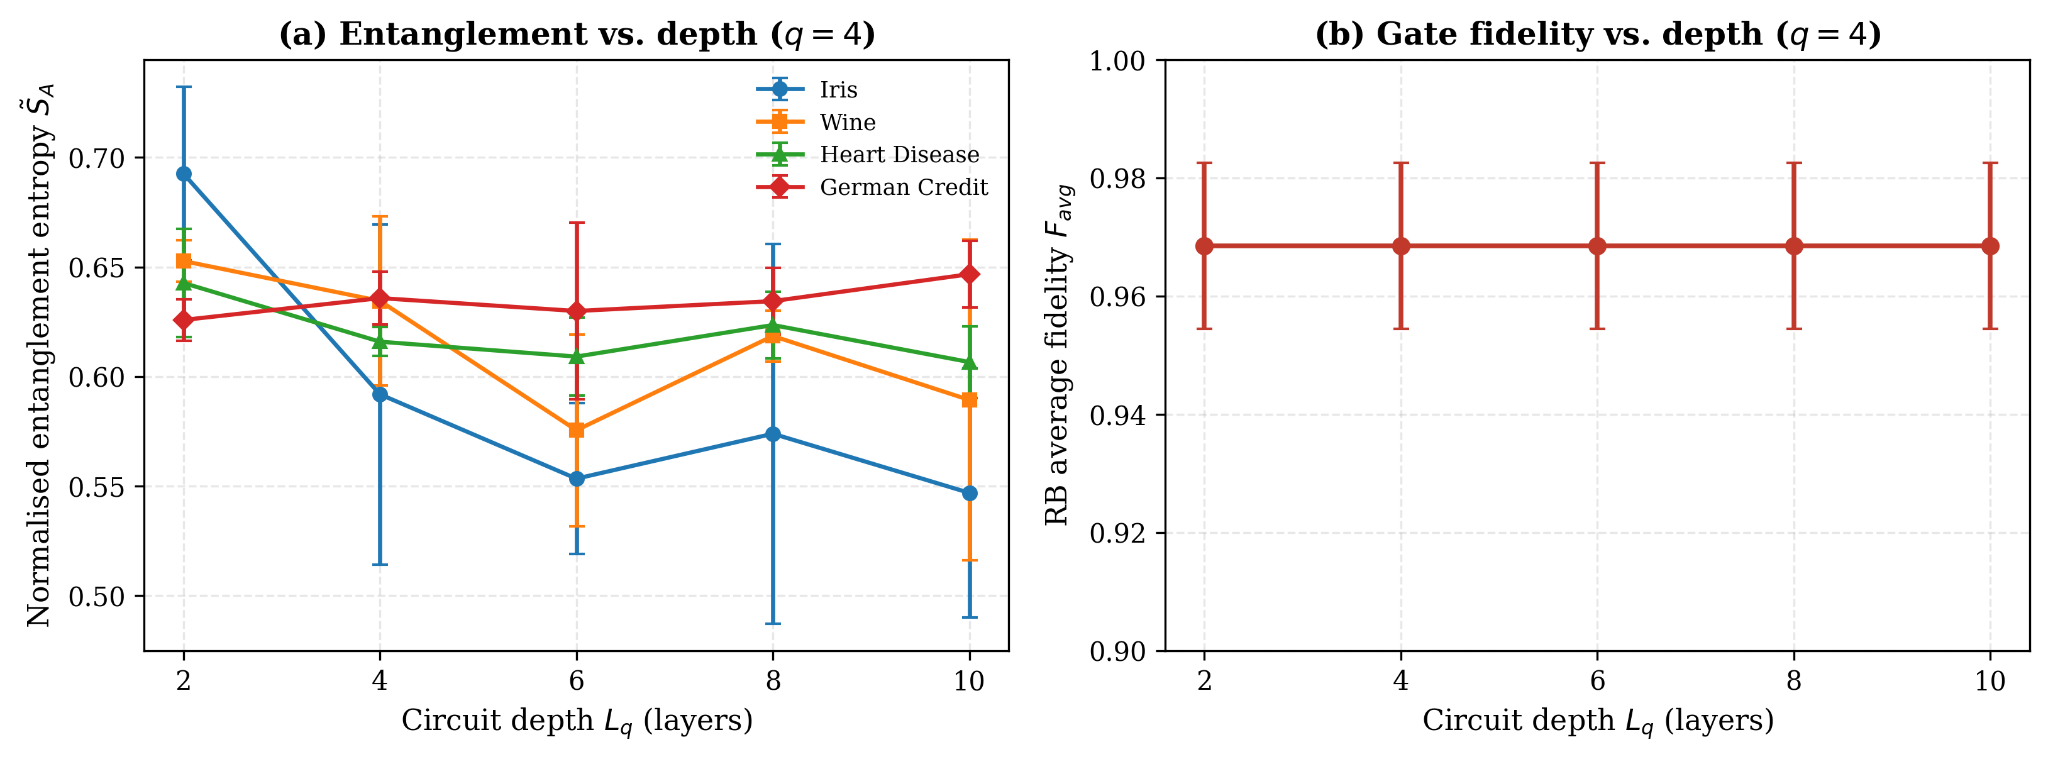
\includegraphics[width=\textwidth]{fig3_depth_scaling_diagnostics.png}}{%
\fbox{\parbox[c][0.22\textheight][c]{0.92\textwidth}{\centering
Missing file \texttt{fig3\_depth\_scaling\_diagnostics.png}.
Upload the figure next to \texttt{Main.tex} on Overleaf.}}}
\caption{Circuit-depth diagnostics at fixed width $q=4$. Panel~(a) reports normalized entanglement entropy as a function of variational depth $L_q$, and Panel~(b) reports the randomized-benchmarking-inspired average fidelity $F_{\mathrm{avg}}$. The results support the interpretation that increasing depth does not provide a systematic diagnostic gain after early saturation.}
\label{fig:depth_scaling_diagnostics}
\end{figure}
\paragraph{Evaluation of entanglement and RB with changing qubits.}\label{subsec:wine_results}

We evaluate how the quantum diagnostics of IPQSSL change as the number of qubits $q$ increases. This analysis studies the trade-off between representational capacity and circuit reliability: more qubits enlarge the Hilbert space and may support richer quantum correlations, but they can also increase circuit complexity and noise sensitivity~\cite{mcclean2018barren,cerezo2021cost,holmes2022connecting}.
We therefore report the normalized bipartite entanglement entropy $\widetilde{S}_A$ and randomized-benchmarking average fidelity $F_{\mathrm{avg}}$. These diagnostics assess whether increasing $q$ produces meaningful entanglement while preserving stable circuit fidelity.

\begin{table}[H]
  \centering
  \caption{Normalized entanglement entropy $\widetilde{S}_A$ (mean $\pm$
  std over seeds) as a function of circuit width $q$ at fixed depth
  $L_q=2$; the $q=4$ column repeats the corresponding column of
  Table~\ref{tab:entropy_rb_depth} for ease of comparison. The
  data-independent per-layer RB average fidelity $F_{\mathrm{avg}}$ is
  reported once per width in the final row; it decreases with $q$
  because each composite layer contains more noisy gates
  (Section~\ref{subsec:rb_fidelity}). Subsystem $A$ comprises the first
  $\lceil q/2\rceil$ qubits (Section~\ref{sec:entropy}).}
  \label{tab:entropy_rb_width}
  \small
  \begin{tabular}{l cccc}
    \toprule
    & $q=4$ & $q=6$ & $q=8$ & $q=10$ \\
    \midrule
    German & $0.6258 \pm 0.0095$ & $0.5639 \pm 0.0324$ & $0.5371 \pm 0.0688$ & $0.4242 \pm 0.0070$ \\
    Heart  & $0.6427 \pm 0.0247$ & $0.5824 \pm 0.0248$ & $0.5231 \pm 0.0318$ & $0.4534 \pm 0.0516$ \\
    Iris   & $0.6926 \pm 0.0397$ & $0.5922 \pm 0.0565$ & $0.5281 \pm 0.0287$ & $0.4582 \pm 0.0744$ \\
    Wine   & $0.6527 \pm 0.0094$ & $0.5937 \pm 0.0473$ & $0.5276 \pm 0.0223$ & $0.4339 \pm 0.0375$ \\
    \midrule
    RB $F_{\mathrm{avg}}$ & $0.9685 \pm 0.0140$ & $0.9452 \pm 0.0061$ & $0.9270 \pm 0.0113$ & $0.9065 \pm 0.0178$ \\
    \bottomrule
  \end{tabular}
\end{table}
\subsection{Entanglement Scaling and Gate-Level Fidelity}
\label{sec:entropy_rb}

At fixed depth $L_q=2$, we examine how the circuit diagnostics change as the
qubit count increases. Table~\ref{tab:entropy_rb_width} and
Figure~\ref{fig:width_scaling_diagnostics} show that
raising $q$ from $4$ to $10$ decreases the dataset-mean normalized
entanglement entropy
from about $0.65$ to $0.44$, while the randomized-benchmarking-inspired
per-layer fidelity decreases from about $0.97$ to $0.91$~\cite{knill2008randomized,magesan2012characterizing,cross2019validating}.
Thus, increasing width is not a free source of quantum structure: under a
fixed-depth ansatz, the generated entanglement becomes diluted across the
larger register, while gate-level error accumulates. These quantities are
therefore used only as circuit diagnostics, not as evidence of quantum
advantage or predictive superiority.

\begin{figure}[H]
\centering
\IfFileExists{fig4_width_scaling_diagnostics.png}{%
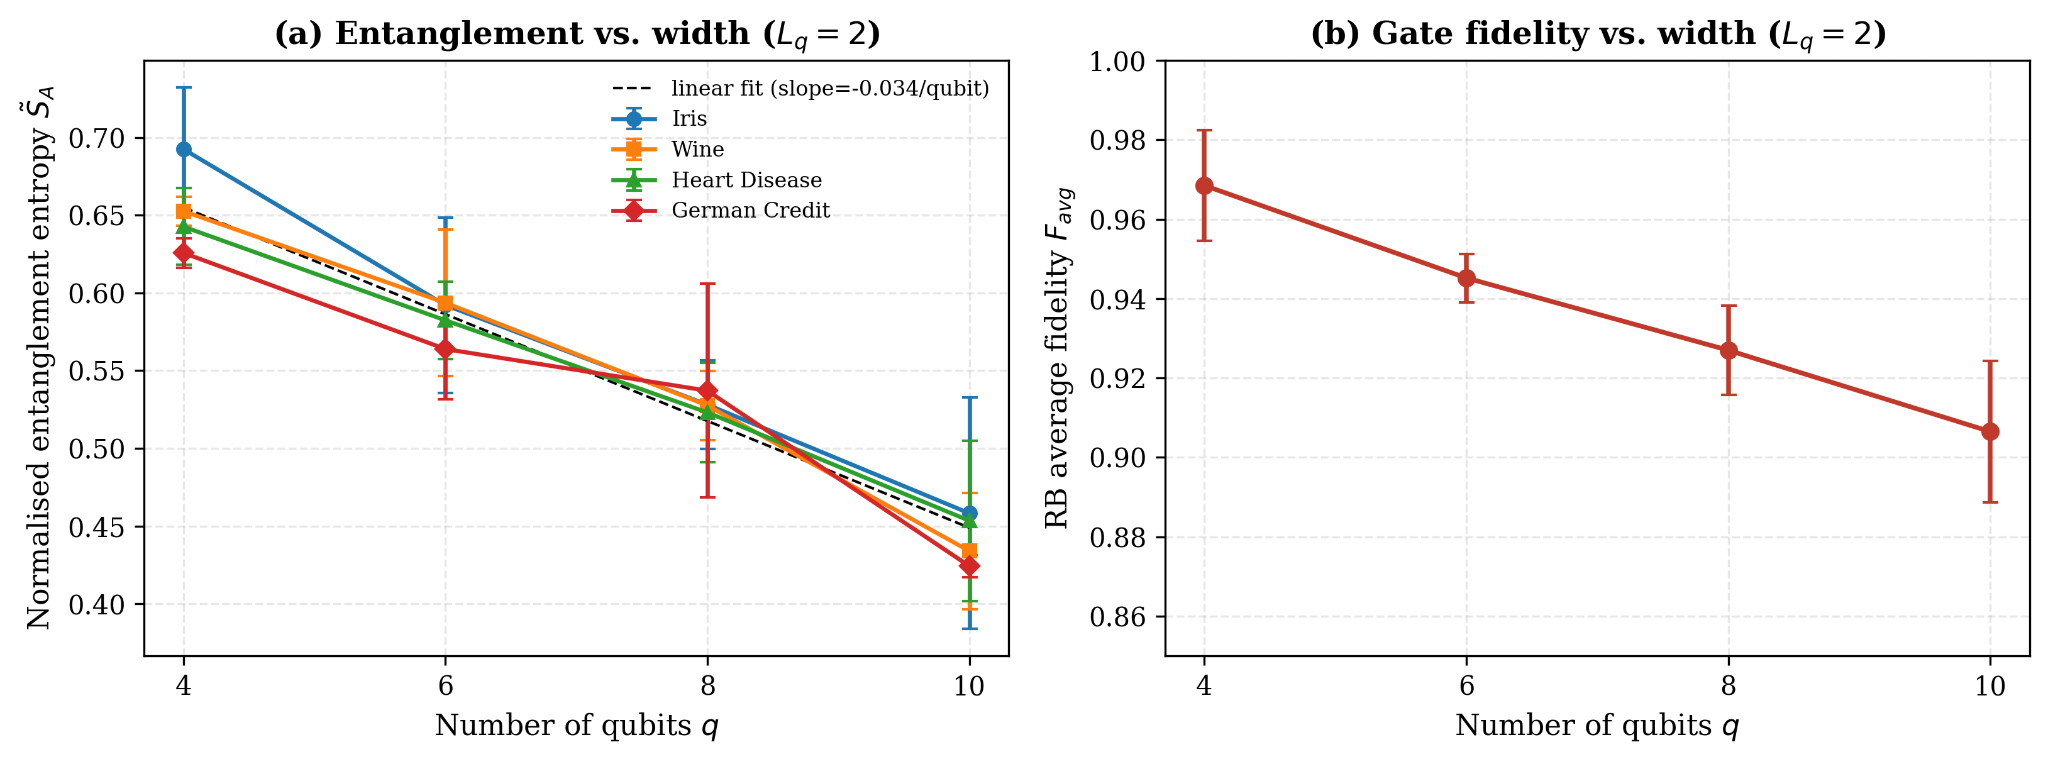
\includegraphics[width=\textwidth]{fig4_width_scaling_diagnostics.png}}{%
\fbox{\parbox[c][0.22\textheight][c]{0.92\textwidth}{\centering
Missing file \texttt{fig4\_width\_scaling\_diagnostics.png}.
Upload the figure next to \texttt{Main.tex} on Overleaf.}}}
\caption{Circuit-width diagnostics at fixed depth $L_q=2$. Increasing the
number of qubits reduces the normalized entanglement entropy and lowers the
randomized-benchmarking-inspired fidelity, illustrating the expressivity--noise
trade-off of the QR-based circuit representation.}
\label{fig:width_scaling_diagnostics}
\end{figure}

% Summary of the Discussion section (for cover letter / response to reviewers / condensed restatement)

\paragraph{ Discussion.}
The Discussion integrates the predictive, ablation, spectral, and
circuit-level findings into a conditional rather than universal claim.
Regularized Poisson propagation with a bounded diagonal term improves upon
Original Poisson when the similarity graph is well aligned with the data
geometry---uniformly on Wine, at three of four budgets on Iris, and, after
budget-dependent crossovers, on Optdigits ($\ell\geq 2$) and Breast Cancer
($\ell=10$)---but not on Heart Disease, German Credit, or Cora. This
dataset- and budget-dependence is itself a finding: diagonal regularization
is not a free improvement.

The five-variant ablation attributes the gains primarily to diagonal
stabilization itself: any bounded nonzero diagonal---random, degree-based,
or circuit-generated---recovers the bulk of the improvement, and supervised
SPSA training of the circuit parameters contributes nothing essentially
under the present protocol. The spectral analysis supplies the mechanism:
at the default, $\alpha_2=0.1$ the unregularized symmetrized operator is
provably indefinite on every dataset, with negative and near-zero
eigenvalues precisely in the low-frequency, label-carrying directions, so
the diagonal term $\mu R$ acts as spectral repair rather than
representation learning. Part of what it repairs is a deficit introduced by
the default $\alpha_2$ itself; the $\alpha_2=0$, $\mu=0$ control arm
required to disentangle sign repair from genuine conditioning improvement
is identified as a necessary completion of the ablation.

The contribution of the quantum component is stated precisely: at the
register sizes considered, the circuit provides a deterministic, bounded,
hardware-compatible inductive bias---not a computational advantage---whose
value is already present at initialization. The circuit-generated weights
are competitive with, but not demonstrably superior to, simpler diagonal
constructions, with the partial exception of the two largest graphs
(Optdigits, Cora), where the \emph{untrained} quantum diagonal attains the
highest mean accuracy among all variants, albeit without statistically
significant separation. The decisive open comparison is a matched-capacity
classical parameterization of the same quadratic form.

Circuit diagnostics favor shallow, narrow circuits: depth saturates early
(accuracy and entanglement entropy are flat beyond $L_q\simeq 6$), while
widening from $q=4$ to $q=10$ dilutes the normalized entanglement from
approximately $0.65$ to $0.44$ and reduces per-layer gate fidelity from
approximately $0.97$ to $0.91$. Five limitations bound the conclusions:
the absence of matched-capacity classical baselines; high split-to-split
variance on Optdigits requiring per-seed analysis; reliance on a single
accuracy metric, with German Credit constituting a negative result for all
propagation methods considered; classical simulation of all quantum
components; and the unquantified share of the ablation gains attributable
to undoing the $\alpha_2$-induced spectral shift.

\section{Conclusion}
\label{sec:conclusion}

The conclusion separates the contributions established by the present theory
and experiments from the quantum capabilities that remain in the pipeline.
We introduced \textsc{IPQSSL}, a quantum-informed regularized Poisson
framework for graph-based semi-supervised classification, and evaluated it
under a protocol designed to separate the contribution of diagonal
stabilization from that of the quantum-generated weights. The contributions
that survive this protocol are the following. On the theoretical side, we
derived a symmetrized, Hermitian, provably block-encoding-compatible
formulation of the regularized Poisson operator, with explicit spectral
conditions for positive definiteness and a clean separation between the
classical NISQ-oriented implementation and a future fault-tolerant
linear-system pathway. On the empirical side, we delineated when diagonal
regularization of the Poisson system helps: consistently on Wine, with
budget-dependent crossovers on Optdigits and Breast Cancer, and not at all
on heterogeneous tabular data or on Cora—and we traced the failure of
the unregularized system to the indefiniteness of the propagation operator
at the standard hyperparameters, so that the regularizer's primary role in
this regime is spectral repair. The ablation shows that this repair is
achieved by generic bounded diagonals as effectively as by trained
quantum-derived ones, and that variational optimization adds nothing under
the present protocol; we report this finding as measured, since an honest
negative delineation is a prerequisite for credible claims of quantum
utility in hybrid graph learning.

Future work follows directly from the limitations. The matched-capacity
classical baselines identified in Section~\ref{subsec:qr_encoding} are the
decisive comparison for the encoding itself, and the positive-definite
$\alpha_2=0$ control arm of
Section~\ref{subsec:diagonal_regularization_ablations} is the cheapest
experiment that would sharpen the causal attribution of the ablation
gains. Per-seed analysis of the
Optdigits bimodality, balanced-accuracy reporting on imbalanced data, and
paired significance testing across the full baseline set would complete
the empirical protocol. On the quantum side, spectrum-aware observables
that target $\lambda_{\min}(\widetilde A_\theta)$ directly, rather than
generic $Z_0$ measurements, would align the circuit output with the
mechanism the ablation shows to matter, and hardware execution of the
shallow $(q,L_q)=(4,2)$ configuration identified by the diagnostics would
replace the simulated fidelity proxy with measured values. The framework's
value is that each of these steps is well-posed: the operator to be
solved, the assumptions under which it block-encodes, and the component of
the pipeline each experiment tests are all stated explicitly.



\section*{Declarations}

\paragraph{Funding.}
Hugo Proen\c{c}a was funded by FCT/MCTES through national funds and by EU
funds under the project UIDB/50008/2020.

\paragraph{Competing interests.}
The authors declare no competing financial or non-financial interests
relevant to the content of this article.

\paragraph{Author contributions.}
 
H.G.\ conceived the framework, designed and implemented the experiments,
performed the formal analysis, prepared all visualisations, and drafted the
manuscript.
F.B.\ contributed to the mathematical formulation and discussion of schemes and reviewed
and edited the manuscript.
H.M.\ contributed to the methodology and reviewed and edited the
manuscript.
H.P., J.N., and M.C.\ provided supervision, project administration, and
revision of the manuscript.
All authors approved the final version of the submitted manuscript.

\paragraph{Data availability.}
The tabular datasets used in this study (Iris~\cite{fisher1988},
Wine~\cite{AeberhardForina1991Wine}, Breast Cancer (Wisconsin
Diagnostic)~\cite{wolberg1995breast}, Heart
Disease~\cite{misc_heart_disease_45}, German Credit~\cite{hofmann1994},
and Optdigits~\cite{alpaydin1998optdigits}) are publicly available from
the UCI Machine Learning Repository. The Cora citation
network~\cite{sen2008collective} is publicly available in the Planetoid
distribution~\cite{yang2016revisiting}.


\paragraph{Code availability.}
The experiment scripts, per-seed result arrays, and figure-generation
code supporting this study are available at
\url{https://github.com/furkanpolaat/IPQSSL}.

\paragraph{Acknowledgements.}
The authors thank MICSS Lab and the University of Antwerp for fostering an
excellent research environment.


\bibliographystyle{unsrtnat}
\bibliography{Main}

\end{document}